\documentclass[onecolumn, compsoc,11pt]{IEEEtran} 
\usepackage{enumitem}
\usepackage{etex}
\usepackage{amssymb,amsfonts,amsmath,amsthm}
\usepackage{graphicx}
\usepackage[usenames,x11names, dvipsnames, svgnames]{xcolor}
\usepackage{amsmath,amssymb}
\usepackage{dsfont}
\usepackage{amsfonts}
\usepackage{mathrsfs}
\usepackage{texshade}
\usepackage{multirow}
\usepackage{hyperref}
\hypersetup{
  colorlinks=true,
  linkcolor=black,
  citecolor=black,
  filecolor=black,
  urlcolor=DodgerBlue4,
  breaklinks=false,
  % linkbordercolor=red,% hyperlink borders will be red
  % pdfborderstyle={/S/U/W 1}% border style will be underline of width 1pt
}
\usepackage{array}
\usepackage{xr}
\usepackage{verbatim}
% \usepackage{multirow}    
% \usepackage[T1,euler-digits]{eulervm}
% \usepackage{times}
% \usepackage{pxfonts}
\usepackage{tikz}
\usepackage{pgfplots}
\usetikzlibrary{shapes,calc,shadows,fadings,arrows,decorations.pathreplacing,automata,positioning}
\usetikzlibrary{external}
\usetikzlibrary{decorations.text}
\usepgfplotslibrary{colorbrewer} 

\tikzexternalize[prefix=./Figures/External/]% activate externalization!
\tikzexternaldisable
% \addtolength{\voffset}{.1in}  
\usepackage{geometry}
\geometry{a4paper, left=.65in,right=.65in,top=.8in,bottom=0.7in}

\addtolength{\textwidth}{-.1in}    
\addtolength{\hoffset}{.05in}    
\addtolength{\textheight}{0in}    
\addtolength{\footskip}{0in}    
\usepackage{rotating}
\definecolor{nodecol}{RGB}{240,240,220}
\definecolor{nodeedge}{RGB}{240,240,225}
\definecolor{edgecol}{RGB}{130,130,130}
\tikzset{%
  fshadow/.style={      preaction={
      fill=black,opacity=.3,
      path fading=circle with fuzzy edge 20 percent,
      transform canvas={xshift=1mm,yshift=-1mm}
    }} 
}
\usetikzlibrary{pgfplots.dateplot}
\usetikzlibrary{patterns}
\usetikzlibrary{decorations.markings}
\usepackage{fancyhdr}
\usepackage{mathtools}
\usepackage{datetime}
\usepackage{comment}
%% ## Equation Space Control---------------------------
\def\EQSP{3pt}
\newcommand{\mltlne}[2][\EQSP]{\begingroup\setlength\abovedisplayskip{#1}\setlength\belowdisplayskip{#1}\begin{equation}\begin{multlined} #2 \end{multlined}\end{equation}\endgroup\noindent}
\newcommand{\cgather}[2][\EQSP]{\begingroup\setlength\abovedisplayskip{#1}\setlength\belowdisplayskip{#1}\begin{gather} #2 \end{gather}\endgroup\noindent}
\newcommand{\cgathers}[2][\EQSP]{\begingroup\setlength\abovedisplayskip{#1}\setlength\belowdisplayskip{#1}\begin{gather*} #2 \end{gather*}\endgroup\noindent}
\newcommand{\calign}[2][\EQSP]{\begingroup\setlength\abovedisplayskip{#1}\setlength\belowdisplayskip{#1}\begin{align} #2 \end{align}\endgroup\noindent}
\newcommand{\caligns}[2][\EQSP]{\begingroup\setlength\abovedisplayskip{#1}\setlength\belowdisplayskip{#1}\begin{align*} #2 \end{align*}\endgroup\noindent}
\newcommand{\mnp}[2]{\begin{minipage}{#1}#2\end{minipage}} 
%% COLOR DEFS------------------------------------------
\newtheorem{thm}{Theorem}
\newtheorem{cor}{Corollary}
\newtheorem{lem}{Lemma}
\newtheorem{prop}{Proposition}
\newtheorem{defn}{Definition}
\newtheorem{exmpl}{Example}
\newtheorem{rem}{Remark}
\newtheorem{notn}{Notation}
%% ------------PROOF INCLUSION -----------------
\def\NOPROOF{Proof omitted.}
\newif\ifproof
\prooffalse % or \draftfalse
\newcommand{\Proof}[1]{
  \ifproof
  \begin{IEEEproof}
    #1\end{IEEEproof}
  \else
  \NOPROOF
  \fi
}
%% ------------ -----------------
\newcommand{\DETAILS}[1]{#1}
%% ------------ -----------------
% color commands------------------------
\newcommand{\etal}{\textit{et} \mspace{3mu} \textit{al.}}
% \renewcommand{\algorithmiccomment}[1]{$/** $ #1 $ **/$}
\newcommand{\vect}[1]{\textbf{\textit{#1}}}
\newcommand{\figfont}{\fontsize{8}{8}\selectfont\strut}
\newcommand{\hlt}{ \bf \sffamily \itshape\color[rgb]{.1,.2,.45}}
\newcommand{\pitilde}{\widetilde{\pi}}
\newcommand{\Pitilde}{\widetilde{\Pi}}
\newcommand{\bvec}{\vartheta}
\newcommand{\algo}{\textrm{\bf\texttt{GenESeSS}}\xspace}
\newcommand{\xalgo}{\textrm{\bf\texttt{xGenESeSS}}\xspace}
\newcommand{\FNTST}{\bf }
\newcommand{\FNTED}{\color{darkgray} \scriptsize $\phantom{.}$}
\renewcommand{\baselinestretch}{.95}
\newcommand{\sync}{\otimes}
\newcommand{\psync}{\hspace{3pt}\overrightarrow{\hspace{-3pt}\sync}}
% \newcommand{\psync}{\raisebox{-4pt}{\begin{tikzpicture}\node[anchor=south] (A) {$\sync$};
%   \draw [->,>=stealth] ([yshift=-2pt, xshift=2pt]A.north west) -- ([yshift=-2pt]A.north east); %\end{tikzpicture}}}
\newcommand{\base}[1]{\llbracket #1 \rrbracket}
\newcommand{\nst}{\textrm{\sffamily\textsc{Numstates}}}
\newcommand{\HA}{\boldsymbol{\mathds{H}}}
\newcommand{\eqp}{ \vartheta }
\newcommand{\entropy}[1]{\boldsymbol{h}\left ( #1 \right )}
\newcommand{\norm}[1]{\left\lVert #1 \right\rVert}%
\newcommand{\abs}[1]{\left\lvert #1 \right\rvert}%
\newcommand{\absB}[1]{\big\lvert #1 \big\rvert}%
% #############################################################
% #############################################################
% PREAMBLE ####################################################
% #############################################################
% #############################################################
% \usepackage{pnastwoF}      
\DeclareMathOperator*{\argmax}{argmax}
\DeclareMathOperator*{\argmin}{arg\,min}
\DeclareMathOperator*{\expect}{\mathbf{E}}
\DeclareMathOperator*{\var}{\mathbf{Var}}

\newcommand{\ND}{ \mathcal{N}  }
\usepackage[linesnumbered,ruled,vlined,noend]{algorithm2e}
\newcommand{\captionN}[1]{\caption{\color{darkgray} \sffamily \fontsize{9}{11}\selectfont #1  }}
\newcommand{\btl}{\ \textbf{\small\sffamily bits/letter}}
\usepackage{txfonts}
% \usepackage{ccfonts}
%%% save defaults
\renewcommand{\rmdefault}{phv} % Arial
\renewcommand{\sfdefault}{phv} % Arial
\edef\keptrmdefault{\rmdefault}
\edef\keptsfdefault{\sfdefault}
\edef\keptttdefault{\ttdefault}

% \usepackage{kerkis}
\usepackage[OT1]{fontenc}
\usepackage{concmath}
% \usepackage[T1]{eulervm} 
% \usepackage[OT1]{fontenc}
%%% restore defaults
\edef\rmdefault{\keptrmdefault}
\edef\sfdefault{\keptsfdefault}
\edef\ttdefault{\keptttdefault}
\tikzexternalenable
% ##########################################################
\tikzfading[name=fade out,
inner color=transparent!0,
outer color=transparent!100]
% ###################################
\newcommand{\xtitaut}[2]{
  \noindent\mnp{\textwidth}{
    \mnp{\textwidth}{\raggedright\Huge \bf \sffamily #1}

    \vskip 1em

    {\bf \sffamily #2}
  }
  \vskip 2em
}
% ###################################
% ###################################
\tikzset{wiggle/.style={decorate, decoration={random steps, amplitude=10pt}}}
\usetikzlibrary{decorations.pathmorphing}
\pgfdeclaredecoration{Snake}{initial}
{
  \state{initial}[switch if less than=+.625\pgfdecorationsegmentlength to final,
  width=+.3125\pgfdecorationsegmentlength,
  next state=down]{
    \pgfpathmoveto{\pgfqpoint{0pt}{\pgfdecorationsegmentamplitude}}
  }
  \state{down}[switch if less than=+.8125\pgfdecorationsegmentlength to end down,
  width=+.5\pgfdecorationsegmentlength,
  next state=up]{
    \pgfpathcosine{\pgfqpoint{.25\pgfdecorationsegmentlength}{-1\pgfdecorationsegmentamplitude}}
    \pgfpathsine{\pgfqpoint{.25\pgfdecorationsegmentlength}{-1\pgfdecorationsegmentamplitude}}
  }
  \state{up}[switch if less than=+.8125\pgfdecorationsegmentlength to end up,
  width=+.5\pgfdecorationsegmentlength,
  next state=down]{
    \pgfpathcosine{\pgfqpoint{.25\pgfdecorationsegmentlength}{\pgfdecorationsegmentamplitude}}
    \pgfpathsine{\pgfqpoint{.25\pgfdecorationsegmentlength}{\pgfdecorationsegmentamplitude}}
  }
  \state{end down}[width=+.3125\pgfdecorationsegmentlength,
  next state=final]{
    \pgfpathcosine{\pgfqpoint{.15625\pgfdecorationsegmentlength}{-.5\pgfdecorationsegmentamplitude}}
    \pgfpathsine{\pgfqpoint{.15625\pgfdecorationsegmentlength}{-.5\pgfdecorationsegmentamplitude}}
  }
  \state{end up}[width=+.3125\pgfdecorationsegmentlength,
  next state=final]{
    \pgfpathcosine{\pgfqpoint{.15625\pgfdecorationsegmentlength}{.5\pgfdecorationsegmentamplitude}}
    \pgfpathsine{\pgfqpoint{.15625\pgfdecorationsegmentlength}{.5\pgfdecorationsegmentamplitude}}
  }
  \state{final}{\pgfpathlineto{\pgfpointdecoratedpathlast}}
}
% ###################################
% ###################################
\newcolumntype{L}[1]{>{\rule{0pt}{2ex}\raggedright\let\newline\\\arraybackslash\hspace{0pt}}m{#1}}
\newcolumntype{C}[1]{>{\rule{0pt}{2ex}\centering\let\newline\\\arraybackslash\hspace{0pt}}m{#1}}
\newcolumntype{R}[1]{>{\rule{0pt}{2ex}\raggedleft\let\newline\\\arraybackslash\hspace{0pt}}m{#1}}




\newcommand{\drhh}[8]{
  \begin{axis}[semithick,
    font=\bf \sffamily \fontsize{7}{7}\selectfont,
    name=H2,
    at=(#4), anchor=#5,
    xshift=.3in,
    yshift=-.3in,
    width=\WDT, 
    height=\HGT, 
    title={{\LARGE G } ROC area distribution (Out-of-sample)}, 
    title style={align=right, },legend cell align=left,
    legend style={ xshift=3.5in, yshift=-.6in, draw=white, fill= gray, fill opacity=0.2, 
      text opacity=1,},
    axis line style={black!80, opacity=0,   thick,,ultra thin, rounded corners=0pt},
    axis on top=false, 
    xlabel={ROC area},
    ylabel={probability},
    ylabel style={yshift=-.25in},
    xlabel style={yshift=.1in},
    grid style={dashed, gray!50},
    % grid,
    axis background/.style={top color=gray!1,bottom color=gray!2},
    enlargelimits=false, 
    scale only axis=true,
    ymin=0,
    % xmin=.7,xmax=1.0,
    ylabel style={yshift=.05in},
    major tick length=0pt,yticklabel style={/pgf/number format/fixed,/pgf/number format/precision=2},xticklabel style={/pgf/number format/fixed,/pgf/number format/precision=2},
    #7,
    ]
    \addplot [
    fill=#8,
    thick,
    draw=white,
    opacity=1,
    hist={density,bins=10},
    ] table [y index=#3] {#1};
    % \addlegendentry{$\Delta$ ROC};
    \addplot [very thick, Red2,, opacity=.95] gnuplot [raw gnuplot] {plot '#1' u #2:(1./#6.) smooth kdensity};
    % 
    % \draw[thin,black ] (axis cs:.89291,\pgfkeysvalueof{/pgfplots/ymin}) -- (axis cs:.89291,\pgfkeysvalueof{/pgfplots/ymax}) node [midway,right, pos=0.2] {89.3\%};
    % \addlegendentry{kde};
  \end{axis}
}


\newcommand{\erhh}[6]{
  \begin{axis}[semithick,
    font=\bf \sffamily \fontsize{7}{7}\selectfont,
    name=H2,
    at=(#3), anchor=#4,
    xshift=.3in,
    yshift=-.3in,
    width=\WDT, 
    height=\HGT, 
    title style={align=center, },legend cell align=left,
    legend style={ xshift=3.5in, yshift=-.6in, draw=white, fill= gray, fill opacity=0.2, 
      text opacity=1,},
    axis line style={black!80, opacity=0,   thick,,ultra thin, rounded corners=0pt},
    axis on top=false, 
    xlabel={ROC area},
    ylabel={probability},
    ylabel style={yshift=-.25in},
    xlabel style={yshift=.1in},
    grid style={dashed, gray!50},
    % grid,
    axis background/.style={top color=gray!1,bottom color=gray!2},
    enlargelimits=false, 
    scale only axis=true,
    % ymin=0, 
    % xmin=.7,xmax=1.0,
    ylabel style={yshift=.05in},
    major tick length=0pt,yticklabel style={/pgf/number format/fixed,/pgf/number format/precision=2},xticklabel style={/pgf/number format/fixed,/pgf/number format/precision=2},
    #5,
    ]
    \addplot[semithick, #6]
    table[x expr=(\coordindex+1),y expr=(\thisrowno{#2})] {#1};
    % \addlegendentry{Cullman, Alabama};
  \end{axis}
}
% ################################################
% ################################################
% ################################################
% ################################################
\def\DISCLOSURE#1{\def\disclosure{#1}}
\DISCLOSURE{\raisebox{15pt}{$\phantom{XxxX}$This sheet contains proprietary information 
    not to be released to third parties except for the explicit purpose of evaluation.}
}
% ####################################
\newcommand{\set}[1]{\left\{ #1 \right\}}
\newcommand{\paren}[1]{\left( #1 \right)}
\newcommand{\bracket}[1]{\left[ #1 \right]}
% \newcommand{\norm}[1]{\left\Vert #1 \right\Vert}
\newcommand{\nrm}[1]{\left\llbracket{#1}\right\rrbracket}
\newcommand{\parenBar}[2]{\paren{#1\,{\left\Vert\,#2\right.}}}
\newcommand{\parenBarl}[2]{\paren{\left.#1\,\right\Vert\,#2}}
\newcommand{\ie}{$i.e.$\xspace}
\newcommand{\addcitation}{\textcolor{black!50!red}{\textbf{ADD CITATION}}}
\newcommand{\subtochange}[1]{{\color{black!50!green}{#1}}}
\newcommand{\tobecompleted}{{\color{black!50!red}TO BE COMPLETED.}}


\newcommand{\pIn}{\mathscr{P}_{\textrm{in}}}
\newcommand{\pOut}{\mathscr{P}_{\textrm{out}}}
\newcommand{\aIn}[1][\Sigma]{#1_{\textrm{in}}}
\newcommand{\aOut}[1][\Sigma]{#1_{\textrm{out}}}
\newcommand{\xin}[1]{#1_{\textrm{in}}}
\newcommand{\xout}[1]{#1_{\textrm{out}}}

\newcommand{\R}{\mathbb{R}} % Set of real numbers
\newcommand{\F}[1][]{\mathcal{F}_{#1}}
\newcommand{\SR}{\mathcal{S}} % Semiring of sets
\newcommand{\RR}{\mathcal{R}} % Ring of sets
\newcommand{\N}{\mathbb{N}} % Set of natural numbers (0 included)


\newcommand{\Pp}[1][n]{\mathscr{P}^+_{#1}}
\renewcommand{\entropy}[1]{\boldsymbol{h}\left ( #1 \right )}



\makeatletter
\pgfdeclarepatternformonly[\hatchdistance,\hatchthickness]{flexible hatch}
{\pgfqpoint{0pt}{0pt}}
{\pgfqpoint{\hatchdistance}{\hatchdistance}}
{\pgfpoint{\hatchdistance-1pt}{\hatchdistance-1pt}}%
{
  \pgfsetcolor{\tikz@pattern@color}
  \pgfsetlinewidth{\hatchthickness}
  \pgfpathmoveto{\pgfqpoint{0pt}{0pt}}
  \pgfpathlineto{\pgfqpoint{\hatchdistance}{\hatchdistance}}
  \pgfusepath{stroke}
}
\makeatother

\pgfdeclarepatternformonly{north east lines wide}%
{\pgfqpoint{-1pt}{-1pt}}%
{\pgfqpoint{10pt}{10pt}}%
{\pgfqpoint{9pt}{9pt}}%
{
  \pgfsetlinewidth{0.7pt}
  \pgfpathmoveto{\pgfqpoint{0pt}{0pt}}
  \pgfpathlineto{\pgfqpoint{9.1pt}{9.1pt}}
  \pgfusepath{stroke}
}

\pgfdeclarepatternformonly{north west lines wide}%
{\pgfqpoint{-1pt}{-1pt}}%
{\pgfqpoint{10pt}{10pt}}%
{\pgfqpoint{9pt}{9pt}}%
{
  \pgfsetlinewidth{0.7pt}
  \pgfpathmoveto{\pgfqpoint{0pt}{9pt}}
  \pgfpathlineto{\pgfqpoint{9.1pt}{-0.1pt}}
  \pgfusepath{stroke}
}
\makeatletter

\pgfdeclarepatternformonly[\hatchdistance,\hatchthickness]{flexible hatchB}
{\pgfqpoint{0pt}{\hatchdistance}}
{\pgfqpoint{\hatchdistance}{0pt}}
{\pgfpoint{1pt}{\hatchdistance-1pt}}%
{
  \pgfsetcolor{\tikz@pattern@color}
  \pgfsetlinewidth{\hatchthickness}
  \pgfpathmoveto{\pgfqpoint{0pt}{\hatchdistance}}
  \pgfpathlineto{\pgfqpoint{\hatchdistance}{0pt}}
  \pgfusepath{stroke}
}    \makeatother


\def\TPR{\textrm{TPR}\xspace}
\def\TNR{\textrm{TNR}\xspace}
\def\FPR{\textrm{FPR}\xspace}
\def\PPV{\textrm{PPV}\xspace}

\usetikzlibrary{arrows.meta}
\usetikzlibrary{decorations.pathreplacing,shapes.misc}
\usepgfplotslibrary{fillbetween}
%\usepackage{tikz-network}
\usetikzlibrary{shapes.geometric}
\usetikzlibrary{math}
\usepgfplotslibrary{colorbrewer} 

\usepackage{textcomp}
\usepackage{colortbl}
\usepackage{array}
\usepackage{courier} 
\usepackage{wrapfig}
\usepackage{pifont}
\usetikzlibrary{chains,backgrounds}
\usetikzlibrary{intersections}
\usetikzlibrary{pgfplots.groupplots}
\usepgfplotslibrary{fillbetween} 
\usetikzlibrary{arrows.meta}
\usepackage{pgfplotstable}
%\usepackage[super,compress,sort,comma]{natbib}
\usepackage{setspace}
\usetikzlibrary{math}
\usetikzlibrary{matrix}
\usepackage{xstring}
\usepackage{xspace}
\usepackage{flushend}
\makeatletter
\renewcommand\section{\@startsection {section}{1}{\z@}%
  {-2ex \@plus -1ex \@minus -.2ex}%
  {1ex \@plus.1ex}%
  {\Large\bfseries\scshape}}
\renewcommand\subsection{\@startsection {section}{1}{\z@}%
  {-2ex \@plus -.25ex \@minus -.2ex}%
  {0.1ex \@plus.0ex}%
  {\fontsize{11}{10}\selectfont\bfseries\sffamily\color{black}}}
\renewcommand\subsubsection{\@startsection {section}{1}{\z@}%
  {0ex \@plus -.5ex \@minus -.2ex}%
  {0.0ex \@plus.5ex}%
  {\fontsize{9}{9}\selectfont\bfseries\itshape\sffamily\color{darkgray}}}
\renewcommand\paragraph{\@startsection {section}{1}{\z@}%
  {-.2ex \@plus -.5ex \@minus -.2ex}%
  {0.0ex \@plus.5ex}%
  {\fontsize{9}{9}\selectfont\itshape\sffamily\color{darkgray}}}
   
 
\makeatother
\makeatletter
\pgfdeclareradialshading[tikz@ball]{ball}{\pgfqpoint{-10bp}{10bp}}{%
  color(0bp)=(tikz@ball!30!white);
  color(9bp)=(tikz@ball!75!white);
  color(18bp)=(tikz@ball!90!black);
  color(25bp)=(tikz@ball!70!black);
  color(50bp)=(black)}
\makeatother
\newcommand{\tball}[1][CadetBlue4]{${\color{#1}\Large\boldsymbol{\blacksquare}}$}
\renewcommand{\baselinestretch}{1}
\renewcommand{\captionN}[1]{\caption{\color{CadetBlue4!50!black} \sffamily \fontsize{9}{10}\selectfont #1  }}
\tikzexternaldisable 
\parskip=6pt
\parindent=0pt
\newcommand{\Mark}[1]{\textsuperscript{#1}}
\pagestyle{fancy}

\newcounter{Dcounter}
\setcounter{Dcounter}{1}
\newcommand{\DQS}[1]{\ifdraftQ
{\marginpar{\tikzexternaldisable \tikz{\node[rounded corners=5pt,draw=none,thick,fill=black!10,font=\sffamily\fontsize{7}{8}\selectfont] {\mnp{.45in} {\color{Red3}\raggedright  \#\theDcounter.~#1}}; }}}\stepcounter{Dcounter}\xspace
\fi}

\newcommand{\qn}[1][i]{\Phi_{#1}}
\newcommand{\D}[1][i]{\mathscr{D}\left ( {\Sigma_#1} \right ) }
\newcommand{\Dx}{\mathscr{D}}
\def\J{\mathds{J}}
\def\M{\omega}
\def\N{\mathds{N}}
\newcommand{\cp}[1][P]{\langle #1 \rangle}
\newcommand{\mem}[1]{\M_{#1}}   
\usepackage{textcomp}
\usepackage{colortbl} 
\usepackage{subfigure}
\usepackage{array}
\usepackage{courier}
\usepackage{setspace}
\usepackage{wrapfig}
\usepackage{calligra}
\usepackage{ulem}
\usepackage{multirow}
\renewcommand{\IEEEbibitemsep}{20pt plus 2pt}
\makeatletter
\IEEEtriggercmd{\reset@font\normalfont\fontsize{11}{12}\selectfont}
\makeatother
\IEEEtriggeratref{1}
\newlength{\bibitemsep}\setlength{\bibitemsep}{.2\baselineskip plus .05\baselineskip minus .05\baselineskip}
\newlength{\bibparskip}\setlength{\bibparskip}{0pt}
\let\oldthebibliography\thebibliography
\renewcommand\thebibliography[1]{%
  \oldthebibliography{#1}%
  \setlength{\parskip}{\bibitemsep}%
  \setlength{\itemsep}{\bibparskip}%
}
\setlength{\bibitemsep}{.3\baselineskip plus .05\baselineskip minus .05\baselineskip}

\usetikzlibrary{chains,backgrounds}
\usetikzlibrary{intersections}
\usepackage[super]{cite} 
\makeatletter \renewcommand{\@citess}[1]{\raisebox{1pt}{\textsuperscript{[#1]}}} \makeatother
\usepackage{xstring}
\usepackage{wasysym}
\usepackage[misc]{ifsym}
\renewcommand{\thesectiondis}{\arabic{section}.}
\renewcommand{\thesubsectiondis}{\arabic{section}.\arabic{subsection}.}

\makeatletter
\renewcommand\section{\@startsection {section}{1}{\z@}%
                                   {-1pt \@plus -30ex \@minus 20ex}%
                                   {.1pt}%
                                   {\large\bfseries\scshape}}
\renewcommand\subsection{\@startsection {subsection}{2}{\z@}%
                                   {0ex \@plus -1.75ex \@minus -1.2ex}%
                                   {0ex \@plus.0ex}%
                                   {\fontsize{11}{11}\selectfont\bfseries\sffamily\color{black}}}
\renewcommand\subsubsection{\@startsection {section}{1}{\z@}%
                                   {-1.5ex \@plus -.5ex \@minus -.2ex}%
                                   {0.0ex \@plus.5ex}%
                                   {\fontsize{9}{9}\selectfont\bfseries\sffamily\color{Red4}}}
\renewcommand\paragraph{\@startsection {section}{1}{\z@}%
                                   {-.1ex \@plus -.5ex \@minus -.2ex}%
                                   {0.0ex \@plus.5ex}%
                                   {\fontsize{11}{10}\selectfont\bfseries\itshape\sffamily\color{black}}}
\makeatother
 
                          
\makeatletter
\pgfdeclareradialshading[tikz@ball]{ball}{\pgfqpoint{-10bp}{10bp}}{%
 color(0bp)=(tikz@ball!30!white);
 color(9bp)=(tikz@ball!75!white);
 color(18bp)=(tikz@ball!90!black);
 color(25bp)=(tikz@ball!70!black);
 color(50bp)=(black)}
\makeatother
\newcommand{\tball}{${\color{CadetBlue3}\Large\boldsymbol{\blacksquare}}$}
\renewcommand{\baselinestretch}{.94}
\newcommand{\VSP}{\vspace{-2pt}}
\renewcommand{\captionN}[1]{\caption{\color{CadetBlue4!80!black} \sffamily \fontsize{9}{10}\selectfont #1  }}
\tikzexternaldisable 
\parskip=6pt
\parindent=0pt
\newcommand{\Mark}[1]{\textsuperscript{#1}}
\lhead{}
\pagestyle{fancy}
\def\COLA{black}
%###################################
\cfoot{\bf\sffamily \scriptsize \color{Maroon!50} I. Chattopadhyay, Department of Medicine, University of Chicago}
\cfoot{}
\rhead{}
%\rhead{\bf\sffamily \scriptsize \color{DodgerBlue4!50} DARPA Young Faculty Award 2017}
%\rhead{\scriptsize\bf\sffamily \href{zed.UChicago.edu}{zed.UChicago.edu}}
%\rfoot{\scriptsize\bf\sffamily\thepage}
\newcommand{\partxt}{\bf\sffamily\itshape}
%############################################################
\newif\iftikzX
\tikzXtrue
\tikzXfalse

\newcommand\guline{\bgroup\markoverwith
{\textcolor{black!30}{\rule[-0.45ex]{2pt}{0.4pt}}}\ULon}
\newcommand\hilit[1]{\textcolor{Red1}{#1}}
\newcommand\hilitx[1]{\guline{#1}}
%############################################################
\addtolength{\voffset}{.1in}
\addtolength{\textwidth}{-.085in}
\addtolength{\hoffset}{.0425in}
\def\PROG{Mallinckrodt\xspace}
\def\ZERO{ACoR\xspace} 
% ############################################################
%###########################################
\def\DXCODES{7,026,942,339}%Number of codes:
\def\uDXCODES{87,627}%Number of unique codes:
\def\RXCODES{}%Number of codes:
\def\uRXCODES{}%Number of unique codes:
\def\numTruven{87 million\xspace}%Number of unique patients in Truven
\def\malesTruven{39270432}%Number of males in Truven
\def\femalesTruven{48112618}%Number of females in Truven
\def\avgLen{}%average length of record
\def\avgNumDX{XX\xspace}%average number of DX codes
\def\avgNumRX{XX\xspace}%average number of DX codes
\def\totalpatients{729,018} %number of unique patients in this study (all cohorts)
\def\totalnpos{729,018} %number of unique patients in this study (all cohorts)
\def\totalnneg{729,018} %number of unique patients in this study (all cohorts)
\def\DXphn{17}%total number of DX phenotypes
\def\RXphn{18}%total number of RX phenotypes
\def\numfeatures{701\xspace}%total number of features used
\def\PREDWINDOW{1}
\def\CONFWINDOW{2}
\def\INFWINDOW{2}
\def\dxcodesM{6462501}% this problem
\def\dxucodesM{17501}% this problem 
\def\dxcodesF{9426722}% this problem 
\def\dxucodesF{18633}% this problem 
%###########################################
\def\acor{ACoR\xspace}

  \def\MXCOL{black}
\def\FXCOL{Orchid3}
\def\MNCOL{SeaGreen4}
\def\FNCOL{SeaGreen4}
\def\NCOL{SeaGreen4}
\def\XCOL{Tomato}
\def\WCOL{Tomato}
\def\YCOL{DodgerBlue4} 
\def\XCOLA{\MXCOL}
\def\XCOLB{\FXCOL}
% ###########################################################
\def\treatment{positive\xspace}
\def\control{control\xspace}



\def\authora{Dmytro Onishchenko}
\def\authorb{Yi Huang}
\def\authorc{James van Horne}
\def\authord{Peter J. Smith}
\def\authore{Michael M. Msall}
\def\authorf{Ishanu Chattopadhyay}

\def\addressa{Department of Medicine, University of Chicago, Chicago, IL USA}
\def\addressb{Committee on Genetics, Genomics \& Systems Biology, University of Chicago, Chicago, IL USA}
\def\addressc{Committee on Quantitative Methods in Social, Behavioral, and Health Sciences, University of Chicago, Chicago, IL USA}
\def\addressd{Department of Pediatrics, Section of Developmental and Behavioral Pediatrics, University of Chicago, Chicago, IL USA}
\def\addresse{Department of Pediatrics, Section Chief of Developmental and Behavioral Pediatrics, University of Chicago, Chicago, IL USA}
\def\addressf{Joseph  P. Kennedy Research Center on Intellectual and Neurodevelopmental Disabilities, University of Chicago, Chicago, IL USA}
\def\addressg{Executive Committee Chair, American Academy of Pediatrics’ Section on Developmental and Behavioral Pediatrics}


\def\TITLE{Reduced False Positives in  Autism Screening Via  Digital  Bio-markers Inferred from Deep Co-morbidity Patterns}
\title{\TITLE}
\author{\sffamily  \fontsize{10}{12}\selectfont  \authora$^{1}$, \authorb$^{1}$, \authorc$^{1}$,  \authord$^{4,7}$, \authore$^{5,6}$ and \authorf$^{1,2,3\bigstar}$\\                                                                
\vspace{10pt}                                                                   
                                                                                
\sffamily  \fontsize{10}{12}\selectfont                                         
$^{1}$\addressa\\   
$^{2}$\addressb\\ 
$^{3}$\addressc\\                                                                    
$^{4}$\addressd\\                            
$^{5}$\addresse\\
$^{6}$\addressf\\
$^{7}$\addressg

\vskip 1em                                                                      
$^\bigstar$To whom correspondence should be addressed: e-mail: \texttt{ishanu@uchicago.edu}.}


\begin{document}
%\tableofcontents


\vspace{20pt}




% Preproposal Narrative (two-page limit): The Preproposal Narrative page limit applies
% to text and non-text elements (e.g., figures, tables, graphs, photographs, diagrams,
% chemical structures, drawings) used to describe the project. Inclusion of URLs that
% provide additional information to expand the Preproposal Narrative and could confer an unfair competitive advantage is prohibited and may result in administrative withdrawal of the pre-application.




% – Research Idea: State the hypothesis to be tested or the objective(s) to be reached.
% State the FY23 ARP Idea Development Award Area(s) of Interest that will be
% addressed. If the proposed project does not address one of the Idea Development
% Award Areas of interest, provide justification that the proposed research addresses a
% critical problem, question, or need in ASD. Detail the ideas and rationale on which
% the proposed project is based. Concisely state the specific aims, provide a brief 
% DOD FY23 Autism Research Program Idea Development Award 13
% overview of the study design including a well-defined population (if applicable) and
% details of the methods to be used. This award cannot be used to conduct clinical
% trials or proof-of-concept intervention studies on human subjects.
% – Impact: Describe the potential impact, both short and long term, of this study on the
% outcomes of individuals with ASD, their families/caregivers, and/or the
% understanding of ASD.
% – Innovation: Describe how the proposed project is innovative and how the research
% represents more than an incremental advance on published data.

% -- Personnel: Clearly describe the ASD expertise of the proposed research team and
% how this will factor into the team’s ability to successfully complete the project.

% SUPPORTING DOC:

% -- References Cited (one-page limit): List the references cited (including URLs if
% available) in the Preproposal Narrative using a standard reference format that includes
% the full citation (i.e., author[s], year published, reference title, and reference source,
% including volume, chapter, page numbers, and publisher, as appropriate).
% – List of Abbreviations, Acronyms, and Symbols: Provide a list of abbreviations,
% acronyms, and symbols used in the Preproposal Narrative.
% – Key Personnel Biographical Sketches (five-page limit per individual): All
% biographical sketches should be uploaded as a single combined file. Biographical
% sketches should be used to demonstrate background and expertise through education,
% positions, publications, and previous work accomplished.


%\section*{Pre-proposal}




\subsection*{Research Idea}
Early diagnosis of Autism Spectrum Disorder (ASD) and  timely  intervention is widely recognized as critical for achieving improved cognitive, behavioral and social outcomes~\cite{hyman2020identification}.
Despite  a growing list of suspected risk factors~\cite{kalb2012determinants,bisgaier2011access,fenikile2015barriers,pmid27565363}, the etiology of Autism is still unclear. Even with increasingly widespread adoption of screening with standardized checklists at 18 and 24 months, the median age of diagnosis for ASD remains at over 4 years.  Starting with a positive initial screen, a clinical diagnosis of ASD is  a  frustrating multi-step process spanning 3 months to 1 year, often delaying  time-critical interventions. One obvious driver for these delays  is the vast number of false positives encountered in the current initial  screening. For example, the  M-CHAT/F, the most widely used  screener~\cite{robins2014validation,hyman2020identification},  produces    over 85 false positives out of every 100   flagged for  diagnostic evaluation, significantly inflating wait times~\cite{pmid27565363} especially in rural and underserved communities.
Further, current  screening tools are sensitive to language barriers and cultural issues, and are  particularly ineffective for children with milder symptoms  with average or above-average cognitive abilities until about school age~\cite{jashar2016cognitive,hyman2020identification}, often due to a ``wait and see'' approach adopted at the primary care. The need for better screening tools is thus paramount.


\begin{wrapfigure}[26]{l}{2.25in}
  \vspace{-40pt}
  
  \hspace{-10pt}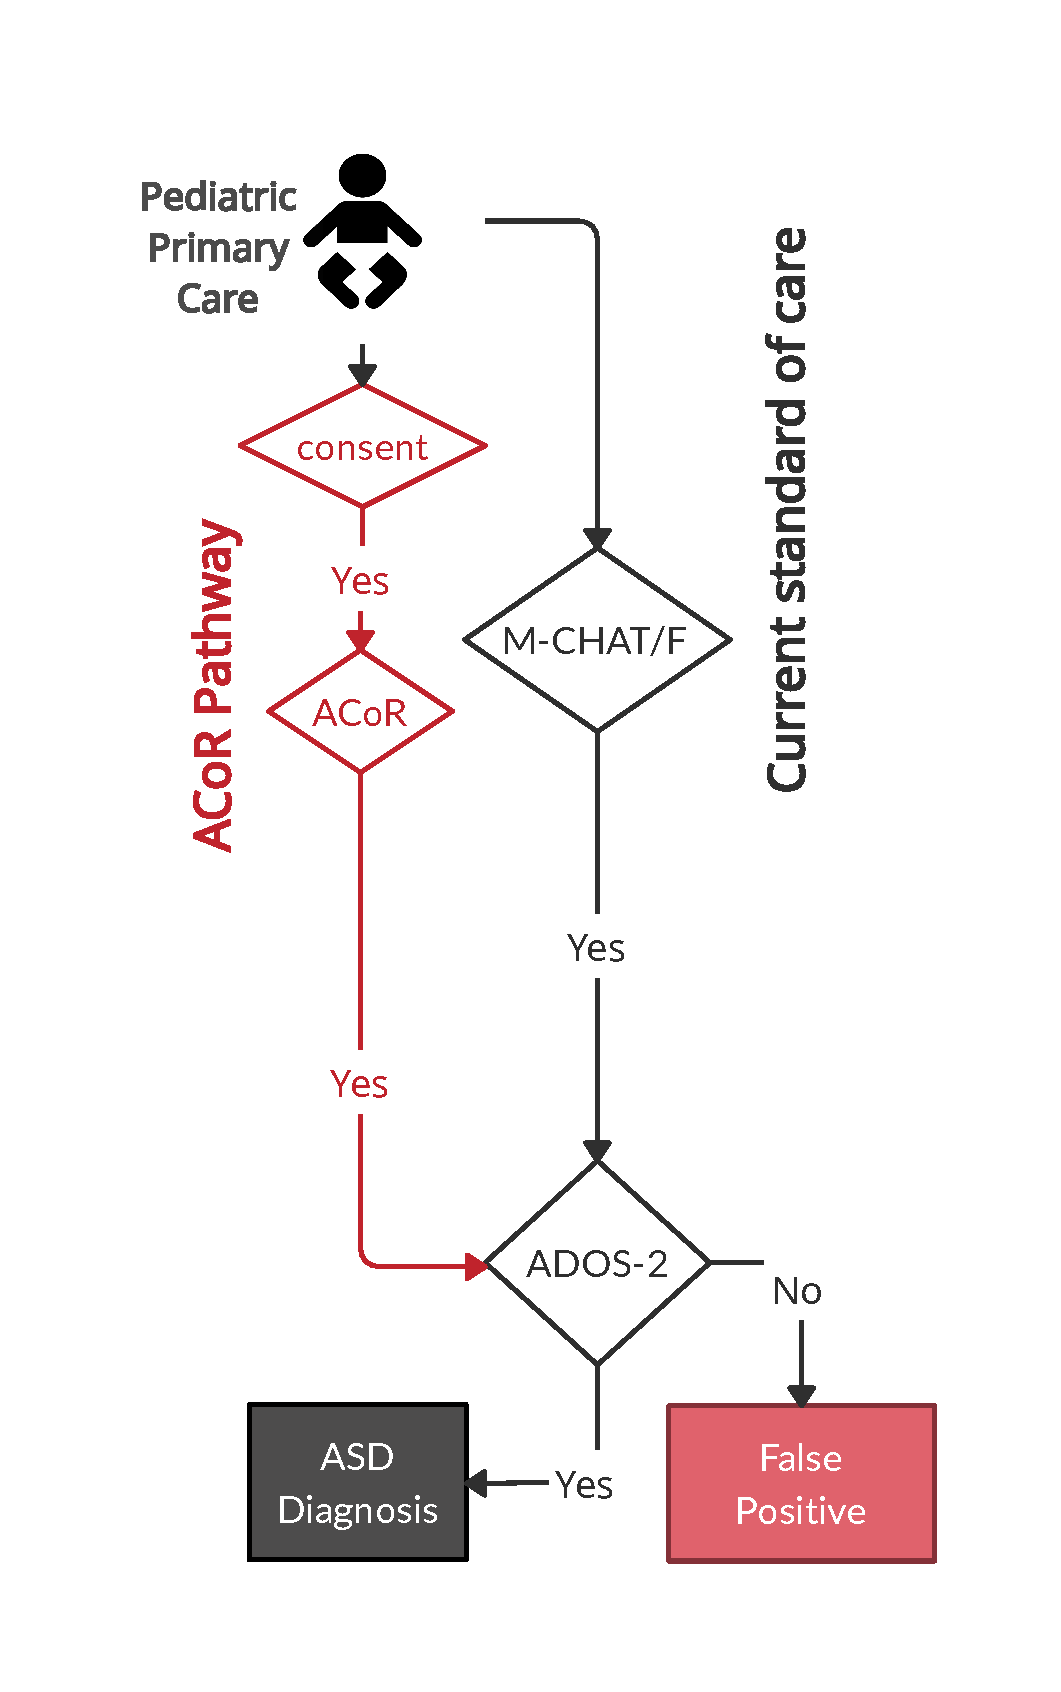
\includegraphics[width=2.75in]{Figures/flowx}
  \vspace{-30pt}
  
  \captionN{Patient processing logic: Note we have parallel pathways through M-CHAT/F and \acor, and
  a flag in either triggers the ADOS-2 evaluation.}\label{figflow}
\end{wrapfigure}%
%
In this study, we plan to validate the efficacy of our recently reported~\cite{Onishchenko_2021}  machine inferred \textbf{digital biomarkers} for autism, prospectively in a  clinical study, carried out in a
pediatric primary care clinic at the University of Chicago. The \textbf{ ASD Co-morbid Risk score (\acor)} uses machine learning (ML)-based pattern discovery on diagnostic codes already present in individual patient files, with no questionnaires and no new laboratory tests or blood-work.. We plan to demonstrate stand-alone \acor efficacy, and compare its effectiveness against existing  tools such as the M-CHAT/F, with children between 16-26 months of age . Our rationale is informed by the extensively documented comorbidities of ASD ranging from dysregulation of immune pathways such as eczema, allergies, asthma, as well as ear and respiratory infections, gastrointestinal problems, developmental issues, severe headaches, migraines, and seizures~\cite{pmid30733689,pmid22511918}. While ASD presentation is highly variable, sophisticated pattern recognition on the longitudinal history of  diagnostic codes is expected to reveal uncharted associations that allow precise screening for at-risk patients.
Orthogonal to  questionnaire based  detection of behavioral signals, the proposed tool potentially reduces socio-economic, ethnic and demographic biases to elicit more  objective and stable results |  with zero  administrative burden on clinicians and parents. With a team comprising machine learning experts, pediatric clinicians and developmental experts with extensive history of research and service in the field (and past collaboration), we hope to demonstrate that \acor can  significantly improve outcomes by either substantially boosting sensitivity  or slashing the false positive rate of the current practice.
%
Thus, the principal study aims are:
     
 \textit{Aim 1: Reduce false positives in current screening protocols.} The current high false positive rate exacerbates post screen wait-time, increasing diagnostic delay. To evaluate the \textit{\guline{hypothesis: \ZERO reduces up to 50\% of false positives}}, we  will track the  cases in which MCHAT-F triggers a flag, but \ZERO does not. Our aim to evaluate the positive predictive value (PPV) of  \ZERO, under high specificity conditions ($>95\%$). Additionally,  evaluate  if \ZERO  replicates high sensitivity observed in preliminary studies without losing specificity.

 \textit{Aim 2. Evaluate the statistical relationship between the \ZERO score and M/CHAT-F, and formalize a joint or conditional operational protocol.} We will characterize statistical association, if any,  between the test scores. \textit{\guline{Hypothesis: The uncertainties or errors in the two tests are are statistically independent.}}  Additionally, we will evaluate our  ability to boost performance by  conditioning the sensitivity-specificity trade-offs on the M-CHAT/F score of individual patients. 

 \textit{Aim 3. Evaluate the effectiveness of \ZERO in a demographically diverse population with a range of socio-economic confounders.} \textit{\guline{Hypothesis: A questionnaire-free approach has the potential to mitigate biases that arise from limitation of language, cultural barriers, and demographic diversity,}} $e.g.$ disproportionately failing  to diagnose children with  average to above-average intelligence in diverse populations~\cite{christensen2019prevalence}, and under-reporting of symptoms by parents or primary care-givers due to cultural differences~\cite{burkett2015african}. 

 \textit{Aim 4. Characterize   heterogeneity of ASD presentation by relating it to patterns in medical history, and predictive co-morbidities.} Heterogeneous presentation  is a key barrier in the mechanistic understanding of ASD pathobiology. \textit{\guline{Hypothesis: We can characterize the distinct classes and/or hierarchies of co-morbidities, by leveraging our ability to disambiguate them  from individual medical histories}}. This will foster new insight  into  intrinsic classes of  the underlying disease processes, and potentially refine/inform intervention design.

    Thus, we are proposing  to exploit observed co-morbidities in children who ultimately meet the criteria for ASD to develop a risk estimation pipeline,  and  predict future clinical  diagnosis  under $2$ years of age. Orthogonal to checklists, we aim to  reduce the median diagnostic age for ASD, by reducing the  long post-screen wait times~\cite{pmid27565363}, by significant boosts in positive predictive value, reduction in false positives, and increased sensitivities at little or no loss of specificity, and \guline{at no additional administrative burden or resource utilization.}

% ####################################
\begin{wrapfigure}[25]{l}{3.65in}
  \vspace{-12pt}
  
  \centering 
   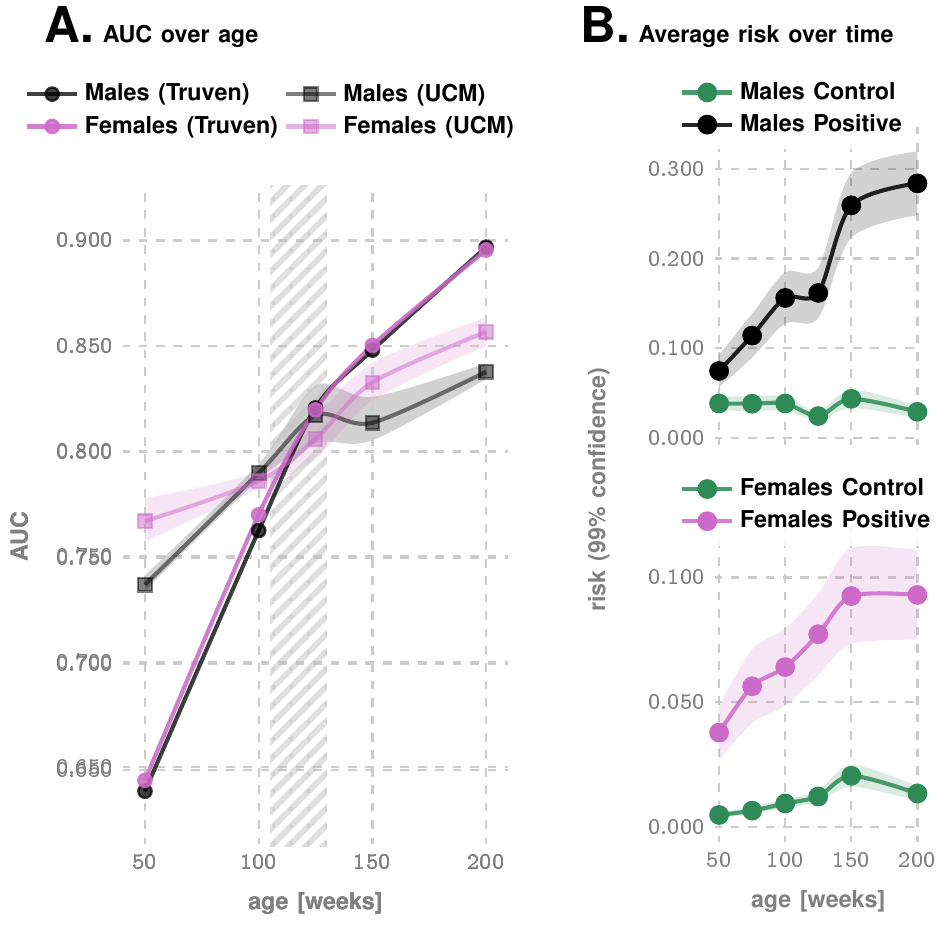
\includegraphics[width=0.5\textwidth]{Figures/perf1}
   \vspace{-15pt}

    \captionN{\acor performance in retrospective studies. Panel A illustrates AUC achieved as a function of
      patient age, for the Truven and UCM datasets: we achieve $>80\%$ AUC for either gender from shortly after 2 years.   Panel B illustrates  risk variation with time for the control and the positive cohorts. % Panel C shows the distribution of the prediction horizon: the time to a clinical diagnosis after inferred  relative risk crosses $90\%$. Panel d illustrates the risk progression of a specific, ultimately autistic male child in the Truven database.
    }\label{fig2}
       \vspace{-15pt}

\end{wrapfigure}
\subsection*{Impact}

A  screening capability  independent of existing tools, deployable as an automated module  of a standard EHR system at the point of care, requiring no behavioral observations or  new blood-work or laboratory tests has considerable  potential to transform ASD care. 

ASD presentation has significant heterogeneity, with no simple comorbidity  consistently signaling future  diagnosis; our algorithms distill robust actionable signatures under such stochastic scenarios. Thus,  \acor opens the possibility of a new screening modality for  neuropsychiatric diseases beyond ASD.
\subsection*{Innovation}
The standardized questionnaires attempt to measure risk by direct observation of behavioral symptoms, as reported by untrained observers (parents). Hence the current screening  tests are only as good as the ability of the questions to discern and disambiguate behavior in infants and toddlers on casual observation, and on the ability of parents and caregivers to correctly interpret and answer the items without bias.
This has lead to possibility of  under-diagnosis in diverse communities as reflected by the
lower apparent prevalence among African-American and Hispanic children. Also, children with average or higher-than-average cognitive abilities seem to have been under-diagnosed as reported is large scale population studies~\cite{hyman2020identification}. Borderline cases are typically problematic to screen for due to the possibility  of subjective interpretation that is built into questionnaire based risk assessment. Responses to checklists are clearly confounded by a host of socio-economic (SES) variables, potential interpretive biases, and  cultural differences. The heterogeneity of presentation also causes issues, since a potential plurality of symptom classes makes it harder for clinicians  to recognize borderline cases, or on-the-fly combine observed co-morbidities with scores from  standardized screening tools. 

In this study, we aim to validate a novel screening tool \acor, which operationalizes a documented aspect of ASD symptomology in  that it has   a wide range  of co-morbidities occurring at  higher rates than in the general population~\cite{hyman2020identification}.
\acor  can potentially address the aforementioned   challenges of ASD screening, by leveraging predictive signatures of  elevated risk gleaned from past medical history of individual  patients alone which are available at the point-of-care, and using no questionnaires, or additional bloodwork or laboratory tests.
\subsection*{Personnel}

\clearpage
 
{\fontsize{9}{10}\selectfont
\bibliographystyle{naturemag}
\bibliography{aut,BibLib1}
}

\end{document}
%#TODO: exclusion and inclusion criteria

\section*{Project Summary}
% 30 line limit
Autism spectrum disorder (ASD) is a developmental disability associated with significant social and behavioral challenges, and there is a distinct need for tools that help identify children with ASD as early as possible. To that effect, we introduce and propose to validate  the ASD Co-morbid Risk (\acor) score in a limited clinical study. The \acor is  computed via sophisticated pattern discovery on longitudinal history of diagnostic codes for individual patients, and potentially signals a future ASD diagnosis within 16-26 months of age. Computation of \acor requires no new blood-work,  or questionnaires, and   uses  data  already available on patient file, with no demand for any particular test or demographic information. Thus, \acor is positioned to be a universal screening tool, that can estimate the risk of autism for all children in a pediatric facility near-instantaneously, potentially outperforming existing tools.  Despite  being  highly heritable,  our  current  incomplete understanding of ASD pathogenesis and the lack of reliable biomarkers hampers early detection, intervention and patient outcomes. The currently available questionnaire based screening tools suffer from vast number of false positives which create long wait-times for diagnostic evaluations. Additionally, standardized checklists are vulnerable  to  socio-economic  and  interpretational  biases  that  disproportionately  impact  diagnosis  in  diverse communities.  Borderline  cases  with  children  with  average  to  above  average  cognitive  abilities  might  be  left undiagnosed till start of school, which negatively impact effectiveness of interventions. The \acor score is designed to   address  the  aforementioned complicated  challenges  of  ASD  screening  by  distilling  incipient    patterns predicting  elevated  risk  from  past medical  history  of  individual  patients. Thus to compute \acor, we operationalize a documented aspect of ASD symptomology in that  it  has  a  wide  range  of  co-morbidities  occurring  at  much  higher  rates  than  in  the  general  population. In  the  setting  of  a  pediatric  primary  care  clinic  at  the  Department  of Pediatrics, University of Chicago, we plan to carry out a comparative study of ACoR with  M-CHAT/F, which is the  most common  screening  tool  in  current  use.  Via  a  direct  comparison,  we  specifically  aim  to  1)  estimate prospectively  to  what  extent  we  can  reduce  false  positives,  2)  the  possibility  of  combining  the  scores  for significant improvements in either Positive Predictive Value or the sensitivity while not losing specificity, 3) the superior  performance  in  ethnically  and  demographically  diverse  cohorts,  and  4)  shed  light  on  the  ASD pathobiology by classifying patterns of co-morbidities that map to  distinct presentations. We have extensively validated our results in retrospective studies on two independent databases of patient records with over four million children. These results  indicate superior performance to existing tools, achieving out-of-sample AUC exceeding  $80\%$ for  either sex from just over 2 years of age. Unlike standard machine learning applications, \acor represents a novel screening modality for ASD, functionaly independent of questionnaires, and potentially can address documented language, cultural and social barriers of the existing tools.
\clearpage

\section*{Project Narrative}
% 2-3 sentence
In contrast to the current questionnaire-based screening tools for autism spectrum disorders (ASD) that suffer from vast amounts of false positives, and a host of demographic, socio-economic and interpretative biases, we aim to validate the ASD Co-morbid Risk (ACoR) score, that estimates ASD risk via sophisticated pattern discovery on the longitudinal medical history of individual patients. Computation of ACoR requires no new blood-work, laboratory tests, questionnaires or psychiatric/cognitive consults, and may be carried out purely from the history of past medical encounters at no additional administrative burden or resource utilization. In addition to stand-alone performance, the combined application of ACoR with currently used functionally independent scores
will be investigated, along with effectiveness in a diverse patient population to assess its ability to address historical under-diagnoses in such communities.

% In contrast to the current questionnaire based screening tools for autism spectrum disorders (ASD) that suffer from vast amounts of false positives, and a host of demographic, socio-economic and interpretative biases, we aim to validate the ASD Co-morbid Risk (\acor) score,  that estimates ASD risk via sophisticated pattern discovery on the longitudinal medical history of individual patients. Computation of \acor requires no new blood-work, laboratory tests, questionnaires or psychiatric/cognitive  consults, and may be carried out purely from the history of past medical encounters at no additional administrative burden or resource utilization. \acor outperforms   the current tool  M-CHAT/F  in  preliminary  studies, and  on  account  of functional independence, the two scores may be combined to further boost performance to either boost positive predictive value up to 100\% or sensitivity up to 50\% with no loss in current specificity.

\clearpage
% ·         3.1, protection of human subjects: You already sent me your draft of this.

% ·         3.2, is this a multi-site study: just needs a yes/no response.

% ·         3.3, data safety monitoring plan: not required because you are not proposing a clinical trial.

% ·         3.4, data safety monitoring board: not required because you are not proposing a clinical trial.

% ·         3.5, team structure: not required because you are not proposing a clinical trial.


\section*{Facilities and Other Resources} 
% add RCC + Memory Center resources

\section*{ACADEMIC PEDIATRICS and
DEVELOPMENTAL AND BEHAVIORAL PEDIATRICS}


University of Chicago Comer Children's Hospital is a 172-bed acute care facility founded in 2005, uniting advanced technology with a family-centered, child-friendly philosophy to provide state-of-the-art care in a six-floor, 242,000-square-feet building. As a major tertiary referral center, Comer Children's sees children with common as well as the most complex medical problems. It admits about 5,000 patients annually from the Chicago area, the Midwest, and around the world. Each year its outpatient clinics accommodate nearly 37,000 general pediatric and specialty visits. Comer Children's is staffed by close to 170 highly trained pediatricians, as well as specially trained nurses and caring support staff, who work together to provide general and specialty medical care for newborns to young adults.

\subsection*{SECTION OF ACADEMIC PEDIATRICS}
The University of Chicago is situated on Chicago’s South Side, a medically underserved area. Our Primary Service area comprises a population of three-quarter of a million people. There is an acute need for primary care practitioners to improve health in the state of Illinois (FY2025 projected shortage -4.0\% and specifically among this population (Chicago South Side Primary Care HPSA score =19). Physicians in this area deliver care that addresses complex medical, psychosocial, and behavioral needs.  They lead efficient, patient-centered primary care practices in underserved communities.

The Section of Academic Pediatrics is dedicated to managing the unique primary care needs of newborns, children and adolescents. The scope of its clinical service covers both the outpatient and inpatient areas located in Comer Children's Hospital and community sites. Its clinical programs include Comer and community hospital medicine, general care nursery, pediatric primary care, Sports Medicine, Child Advocacy and Protective Services and the Comer Mobile Unit.  To support this grant, we will leverage our academic institution and its expanding clinical network across Chicago’s South Side, as well as neighboring federally qualified health centers, to provide diverse and complementary experiences in team-based care. Dr. James Mitchell is the Medical Director for patient services.  

Our provider network includes community health centers and Federally Qualified Health Centers (FQHCs). Sites will include: Comer Children’s Hospital General Pediatrics Clinic, Friend Family Health Center, Erie Family Health Center, ACCESS Community Health Network, and Asian Human Services. All sites have Health Professional Shortage Area designation with scores of 19-21. Some of patient volume statistics are provided as follows:

\textbf{Comer Children's Hospital General Pediatrics Clinic}, located on the University of Chicago Medical campus, serves approximately 12,000 pediatric patients over 22,000 visits annually. Approximately 56% of the patients reside in the South Side community and 35% are insured by Medicaid. This clinic comprises nine pediatricians and one advanced practice nurse.   

\textbf{The Friend Family Health Center} is a large, multi-site Federally Qualified Health Center.   It has served as the primary ambulatory training site for University of Chicago Pediatrics Residency Program since the 1990s.  Friend Health serves over 27,000 patients from Chicago's South Side as part of its mission to provide access to high quality, comprehensive health care   

\textbf{The Erie Family Health Center}, a Federally Qualified Health Center with seven primary care centers and five school-based health centers, provides care to more than 74,000 patients over 300,000 visits annually. These health centers cares for patients across 62 languages. The patient population is 71% Hispanic, with 45% best serviced in a language that is not English. Erie applies team-based care models within their health centers.    

\textbf{ACCESS Community Health Network}, a large Federally Qualified Health Center with 35 health centers across Chicago, cares for more than 183,000 patients per year. ACCESS services the largest proportion of Medicaid beneficiaries in Illinois.  

\textbf{Asian Human Services (AHS)} is a multi-site Federally Qualified Health Center which services a largely immigrant population. AHS provides comprehensive care to more than 30,000 people from more than 55 countries.


\subsection*{THE SECTION OF DEVELOPMENTAL AND BEHAVIORAL PEDIATRICS (DBP)}
The Section of DBP is a Center of Excellence in developmental diagnosis, biomedical management and family supports for children with motor, communicative, sensory, developmental, genetic, neurological, learning and behavior disorders. The section’s goals are to:
\begin{itemize}

\item Promote the highest quality interdisciplinary assessment and biopsychosocial management practices to optimize child functioning, support families and maximize prevention strategies across health, education and community care systems.
\item  Provide the necessary leadership to ensure that children with complex challenges have a high quality medical home and that best practices are used to improve their ability to communicate, move, regulate behavior, interact socially, learn functional and adaptive skills, perform in school and participate in the community.  
\item Serve as a resource for primary care practitioners and pediatric subspecialists for children with the highest biomedical and psychosocial risks associated with suboptimal educational outcomes. • \item Serve as a resource for community professionals and agencies for children with developmental delays, complex disorders after prematurity, genetic, neurological, or cardiopulmonary disorders or experiencing complex behavioral challenges after life-threatening illnesses. . 
\item Enhance training and research so families will benefit from the best clinical and scientific advances with the highest standards of ethics, professionalism and advocacy. 
\item For children with complex medical and/or behavioral challenges and for families with psycho-social or economic stress, DBP provides interventions and assistance. Many of these children and families require teamwork and leadership to promote their health, development, and social competencies. DBP physicians take into account the entire family dynamic and provide guidance in securing ancillary therapies, support services and special school considerations as needed.  
\item We have the clinical expertise coupled with research, educational; advocacy and public policy activities needed for insuring that children receiving translational technologies have information and supports for long term success. Our scope and leadership roles are recognized at the local, regional, national and international levels. We have established clinical, advocacy and research cooperative activities with specialists in community pediatrics, child and adolescent psychiatry, neonatology, critical care medicine, genetics, neurology, child protective services, developmental psychology, public policy and social sciences. These collaborations are not limited to the University of Chicago campus, but extend to other institutions nationally and internationally. Our activities are complementary to those of our collaborators—bringing cross-fertilization of ideas to bear on topics of life course outcomes of children with prematurity. Our Section’s activities are interdisciplinary and include faculty from Public Policy, Social Sciences and Economics to work towards our common interests in improving the quality of life for children with disabilities. 
\end{itemize}

\textbf{The Woodlawn Center} is the clinical home of DBP. It is a site for clinical evaluation and research that can accommodate patients 6 days a week with two exam rooms, equipped to provide developmental assessments from 0-18 years of age. The focus at the Woodlawn Center is on early developmental and cognitive assessments that provide early definition of school-age diagnosis and both clinical and educational needs. 

Interdisciplinary professionals at this center include speech and occupational therapists, social work, developmental psychology, and community outreach professionals.   We provide Autism Diagnostic Observation Schedule (ADOS) testing for accurately assessing and diagnosing autism spectrum disorders.  ADOS is a standardized diagnostic test which provides information on communication, social interaction, and play (or imaginative use of materials) for individuals suspected of having autism or other pervasive developmental disorders, and, as appropriate, provide access to services which may be recommended for each child. .  

DBP and the \textbf{Pediatric Neuropsychology Service} both maintain up to date assessment protocols and manuals for the interdisciplinary assessment of children’s motor, manipulative, conceptual, cognitive, behavioral, and educational skills. These include all the assessment instruments specified in the neurodevelopmental assessment protocol for children in this study. These assessment tools have been used by health professionals representing developmental pediatrics, developmental psychology, physical therapy, occupational therapy, speech language pathology, and special education. A specialized library of current assessment references as well as audiovisual and computer assisted training materials are available.  The Pediatric Neuropsychology Service is a clinical, training and research program within the Section of Child and Adolescent Psychiatry, in the Department of Psychiatry.  The Service provides assessment and Diagnostic services for infants and children with neurodevelopmental learning, emotional regulation and medical disorders and conditions.  The service is also involved in collaborative clinical research, examining the neurocognitive and behavioral sequelae of a wide range of disorders.  



\vskip 1em

\hrule

\section*{Computational Facilities}


The principal investigators have access to extensive computational facilities available at the University of Chicago to carry out the tasks described.


\textbf{Access to Clinical Data for AI-enabled Analytics:} The ZeD lab (overseen by Professor Chattopadhyay) is housed within the Department of Medicine at the University of Chicago, and has access to the full range of high end computing resources offered by the University of Chicago. In addition, Prof. Chattppadyay's laboratory has access to the HIPAA compliant clinical data warehouse maintained by the Biological Sciences Division as detailed below:

\textbf{The Clinical Research Data Warehouse:} (CRDW) within the Biomedical Sciences Division of the University of Chicago is one of the deepest, richest, and most research-ready data repositories of its kind. Containing more than a decade of University of Chicago medical data, it seamlessly brings together multiple internal and external data sources to provide researchers with access to more than 12 million encounters for 2.3 million patients. The associated diagnoses, labs, medications, and procedures number in the tens of millions each. The CRDW is run on IBM Netezza Pure Data System for Analytics servers, a patented Asymmetric Massively Parallel Processing architecture designed to deliver exceptional query performance and modular scalability on highly complex mixed workloads.

In order to meet the acute need for data related to COVID-19, the CRDW team has constructed three data marts (de-identified, limited, and identified) to provide the most commonly requested data elements for this patient population. The initial instance of the COVID-19 data mart includes de-identified structured data on patient demographics, encounters, diagnoses, labs, medications, flow sheets, and procedures. Additional data will be added based on resource availability and urgency.

\textbf{Cohort Discovery Tool:} The purpose of this tool (SEE Cohorts) is to provide a secure web-based tool for the initial exploration of de-identified data. It allows researchers to search available data, build a cohort of patients, and view actual de-identified data within the interface. The data in SEE Cohorts is refreshed weekly.

\textbf{Research Computing Center:} The University of Chicago Research Computing Center (RCC) provides high-end research computing resources to researchers at the University of Chicago, which include high-performance computing and visualization resources; high-capacity storage and backup; software; high-speed networking; and hosted data sets. Resources are centrally managed by RCC staff who ensure the accessibility, reliability, and security of the compute and storage systems. A high-throughput network connects the Midway Compute Cluster to the UChicago campus network and the public internet through a number of high-bandwidth uplinks. To support data-driven research RCC hosts a number of large datasets to be accessed within the RCC compute environment.

RCC maintains three pools of servers for distributed high-performance computing. Ideal for tightly coupled parallel calculations, tightly-coupled nodes are linked by a fully non-blocking FDR-10 Infiniband interconnect. Loosely-coupled nodes are similar to the tightly-coupled nodes, but are connected with GigE rather than Infiniband and are best suited for high-throughput jobs. Finally,  shared memory nodes contain much larger main memories (up to 1 TB) and are ideal for memory-bound computations. The types of CPU architectures RCC maintains are tabulated in Table~\ref{tabcap}.

\begin{table}
\captionN{University of Chicago Research Computing Center Capabilities Summary}\label{tabcap}
\setlength{\arrayrulewidth}{1pt}
\bf\sffamily\fontsize{9}{10}\selectfont
\begin{tabular}{||C{.8in}|c|R{1.85in}|R{.5in}|c||}\hline
\rowcolor{SeaGreen1}Cluster	&Partition&	Compute cores (CPUs)&	Memory	&Other configuration details\\\hline
midway1	&westmere&	12 x Intel X5675 3.07 GHz&	24 GB	& \\\hline
 	&sandyb	&16 x Intel E5-2670 2.6GHz&	32 GB	& \\\hline
 &	bigmem&	16 x Intel E5-2670 2.6GHz&	256 GB	& \\\hline
 	& &	32 x Intel E7-8837 2.67GHz&	1 TB&	 \\\hline
 	&gpu&	16 x Intel E5-2670 2.6GHz&	32 GB&	2 x Nvidia M2090 or K20 GPU\\\hline
 &	 &	20 x Intel E5-2680v2 2.8GHz&	64 GB&	2 x Nvidia K40 GPU\\\hline
 &	mic&	16 x Intel E5-2670 2.6GHz&	32 GB&	2 x Intel Xeon Phi 5100 coprocessor\\\hline
 &	amd&	64 x AMD Opteron 6386 SE&	256 GB&	 \\\hline
 &	ivyb&	20 x Intel E5-2680v2 2.8GHz&	64 GB&	 \\\hline
midway2&	broadwl&	28 x Intel E5-2680v4 2.4GHz&	64 GB&	 \\\hline
 &	bigmem2&	28 x Intel E5-2680v4 @ 2.4 GHz&	512 GB	 &\\\hline
 	&gpu2&	28 x Intel E5-2680v4 @ 2.4 GHz&	64 GB&	4 x Nvidia K80 GPU\\\hline
\end{tabular}
\end{table}


RCC also maintains a number of specialty nodes: 
\begin{itemize}
\item \textit{\color{gray} Large shared memory nodes} - up to 1 TB of memory per node with either 16 or 32 Intel CPU cores. Midway is always expanding, but at time of writing RCC contains a total of 13,500 cores across 792 nodes, and 1.5 PB of storage.
\item  \textit{\color{gray}  Hadoop:} Originally developed at Google, Hadoop is a framework for large-scale data processing.   \item  \textit{\color{gray}  GPU Computing:} Scientific computing on graphics cards can unlock even greater amounts of parallelism from code. RCC GPU nodes each include two Nvidia Tesla-class accelerator cards and are integrated in the Infiniband network. RCC currently provides access to Fermi-generation M2090 GPU devices and Kepler-generation K20 and K40 devices.  \item  \textit{\color{gray}  Xeon Phi:} The Many Integrated-Core architecture (MIC) is Intel's newest approach to manycore computing. Researchers can experiment with these accelerators by using  MIC nodes, each of which have two Xeon Phi cards, and are integrated into the Infiniband network.
\end{itemize}

\textbf{Persistent and High-Capacity Storage.} Storage is accessible from all compute nodes on Midway1 and Midway2 as well as outside of the RCC compute environment through various mechanisms, such as mounting directories as network drives on your personal computer or accessing data as a Globus Online endpoint (at the time of this writing, Globus Online is supported on Midway1). RCC takes snapshots of all home directories (users' private storage space) at regular intervals so that if any data is lost or corrupted, it can easily be recovered. RCC maintains GPFS Filesystem Snapshots for quick and easy data recovery.  In the event of catastrophic storage failure, archival tape backups can be used to recover data from persistent storage locations on Midway. Automated snapshots of the home and project directories are available in case of accidental file deletion or other problems. Currently snapshots are available for these time periods: 1) 7 daily snapshots, 2) 4 weekly snapshots.

\textbf{Tape Backups.} Backups are performed on a nightly basis to a tape machine located in a different data center than the main storage system. These backups are meant to safeguard against events such as hardware failure or disasters that could result in the complete loss of RCC’s primary data center.


\textbf{Data Sharing.} All data in RCC's storage environment is accessible through a wide range of tools and protocols. Because RCC provides centralized infrastructure, all resources are accessible by multiple users simultaneously, which makes RCC’s storage system ideal for sharing data among your research group members. Additionally, data access and restriction levels can be put in place on an extremely granular level.

\textbf{Data Security \& Management.} The HIPAA compliant security of the Research Computing Center’s storage infrastructure, protected by two-factor authentication,  gives users peace of mind that their data is stored, managed, and protected by HPC professionals. Midway's file management system allows researchers to control access to their data. RCC has the ability to develop data access portals for different labs and groups.



\clearpage

%Authentication of Key Biological and Chemical Resources
%If the Research Strategy does not propose use of key biological and/or %chemical resources, the Authentication attachment may include a brief %statement indicating that no key biological and/or chemical resources %will be used in the activities proposed in the application

%Resource Sharing Plan

%PHS Human Subjects and Clinical Trials Information

%enrollment report

%letters of support

%study section assignment?



\section{Cover Page}
\clearpage
$\phantom{x}$
\vspace{-35pt}  
\section{Specific Aims}
Early diagnosis of Autism Spectrum Disorder (ASD) and  timely  intervention is widely recognized as critical for achieving improved cognitive, behavioral and social outcomes~\cite{hyman2020identification}.
Despite  a growing list of suspected risk factors~\cite{kalb2012determinants,bisgaier2011access,fenikile2015barriers,pmid27565363}, the etiology of Autism is still unclear. Even with increasingly widespread adoption of screening with standardized checklists at 18 and 24 months, the median age of diagnosis for ASD remains at over 4 years.  Starting with a positive initial screen, a clinical diagnosis of ASD is  a  frustrating multi-step process spanning 3 months to 1 year, often delaying  time-critical interventions. One obvious driver for these delays  is the vast number of false positives encountered in the current initial  screening. For example, the  M-CHAT/F, the most widely used  screener~\cite{robins2014validation,hyman2020identification},  produces    over 85 false positives out of every 100   flagged for  diagnostic evaluation, significantly inflating wait times~\cite{pmid27565363} especially in rural and underserved communities.
Further, current  screening tools are sensitive to language barriers and cultural issues, and are  particularly ineffective for children with milder symptoms  with average or above-average cognitive abilities until about school age~\cite{jashar2016cognitive,hyman2020identification}, often due to a ``wait and see'' approach adopted at the primary care. The need for better screening tools is thus paramount.


In this study, we plan to validate the efficacy of our recently reported~\cite{Onishchenko_2021}  machine inferred \textbf{digital biomarkers} for autism, prospectively in a limited clinical study, carried out in a
pediatric primary care clinic at the University of Chicago. The \textbf{ ASD Co-morbid Risk score (\acor)} uses machine learning (ML)-based pattern discovery on diagnostic codes already present in individual patient files. We plan to demonstrate stand-alone \acor efficacy, and compare its effectiveness against existing  tools such as the M-CHAT/F, with children between 16-26 months of age . Our rationale is informed by the extensively documented comorbidities of ASD ranging from dysregulation of immune pathways such as eczema, allergies, asthma, as well as ear and respiratory infections, gastrointestinal problems, developmental issues, severe headaches, migraines, and seizures~\cite{pmid30733689,pmid22511918}. While ASD presentation is highly variable, sophisticated pattern recognition on the longitudinal history of  diagnostic codes is expected to reveal uncharted associations that allow precise screening for at-risk patients.
Orthogonal to  questionnaire based  detection of behavioral signals, the proposed tool potentially reduces socio-economic, ethnic and demographic biases to elicit more  objective and stable results |  with zero  administrative burden on clinicians and parents. With a team comprising machine learning experts, pediatric clinicians and developmental experts with extensive history of research and service in the field (and past collaboration), we hope to demonstrate that \acor can  significantly improve outcomes by either substantially boosting sensitivity  or slashing the false positive rate of the current practice.
%
Thus, the principal study aims are:
     
\begin{enumerate} 
[label=$\square$, leftmargin=0pt,
labelindent=0em, topsep=0.1em, labelsep=*, itemsep=.5em,itemindent=1em]
 \item \textbf{Aim 1: Reduce false positives in current screening protocols.} The current high false positive rate exacerbates post screen wait-time, increasing diagnostic delay. To evaluate the \textit{\guline{hypothesis: \ZERO reduces up to 50\% of false positives}}, we  will track the  cases in which MCHAT-F triggers a flag, but \ZERO does not. Our aim to evaluate the positive predictive value (PPV) of  \ZERO, under high specificity conditions ($>95\%$). Additionally,  evaluate  if \ZERO  replicates high sensitivity observed in preliminary studies without losing specificity.

\item \textbf{Aim 2. Evaluate the statistical relationship between the \ZERO score and M/CHAT-F, and formalize a joint or conditional operational protocol.} We will characterize statistical association, if any,  between the test scores. \textit{\guline{Hypothesis: The uncertainties or errors in the two tests are are statistically independent.}}  Additionally, we will evaluate our  ability to boost performance by  conditioning the sensitivity-specificity trade-offs on the M-CHAT/F score of individual patients. 
%
\item \textbf{Aim 3. Evaluate the effectiveness of \ZERO in a demographically diverse population with a range of socio-economic confounders.} \textit{\guline{Hypothesis: A questionnaire-free approach has the potential to mitigate biases that arise from limitation of language, cultural barriers, and demographic diversity,}} $e.g.$ disproportionately failing  to diagnose children with  average to above-average intelligence in diverse populations~\cite{christensen2019prevalence}, and under-reporting of symptoms by parents or primary care-givers due to cultural differences~\cite{burkett2015african}. 

  \item \textbf{Aim 4. Characterize   heterogeneity of ASD presentation by relating it to patterns in medical history, and predictive co-morbidities.} Heterogeneous presentation  is a key barrier in the mechanistic understanding of ASD pathobiology. \textit{\guline{Hypothesis: We can characterize the distinct classes and/or hierarchies of co-morbidities, by leveraging our ability to disambiguate them  from individual medical histories}}. This will foster new insight  into  intrinsic classes of  the underlying disease processes, and potentially refine/inform intervention design.
  \end{enumerate}
Thus, we are proposing  to exploit observed co-morbidities in children who ultimately meet the criteria for ASD to develop a risk estimation pipeline,  and  predict future clinical  diagnosis  under $2$ years of age. Orthogonal to checklists, we aim to  reduce the median diagnostic age for ASD, by reducing the  long post-screen wait times~\cite{pmid27565363}, by significant boosts in positive predictive value, reduction in false positives, and increased sensitivities at little or no loss of specificity, and \guline{at no additional administrative burden or resource utilization.}
\clearpage

\section{Research Strategy}
\parskip=8pt
\setcounter{page}{1}
\begin{wrapfigure}[8]{r}{2.5in}
  \bf \sffamily \fontsize{8}{8}\selectfont
  \vspace{-10pt}
  \centering
  
  \textbf{Abbreviations Used}
  \vskip .5em
  \hspace{-10pt}
  \begin{tabular}{|R{.6in}|L{1.55in}|}\hline
  \rowcolor{lightgray} ASD & Autism Spectrum Disorder\\
  \rowcolor{lightgray!50}M-CHAT/F & Modified Checklist for Autism in Toddlers with Followup\\
 \rowcolor{lightgray} ADOS / ADOS-2 & Autism Diagnostic Observation Schedule \\
  \rowcolor{lightgray!50}EHR  & Electronic Health Records \\
 \rowcolor{lightgray} {\color{Red3} ACoR} & {\color{Red3} Autism Comorbid Risk score} \\\hline
\end{tabular}
\end{wrapfigure}
\subsection{Significance}
Autism spectrum disorder is a developmental disability associated with significant social and behavioral challenges.  The prevalence of ASD  has risen dramatically in the United States from 1-in-10,000 in
 1972 to 1-in-59 children in 2014, to 1-in-44 in 2021, with males  diagnosed at nearly four times the rate of females~\cite{pmid29701730,cdc}.
There is a current lack of   consensus on whether increased awareness and recent changes in diagnostic practices~\cite{hyman2020identification} can fully explain this  trend~\cite{pmid19737791}. Nevertheless, with   possibly  over 1\% of individuals affected worldwide~\cite{pmid22495912},  ASD is  a human condition with potentially serious negative impacts on individuals, families, and communities. 
Early detection  improves outcomes~\cite{hyman2020identification}, is of paramount importance when designing interventions, and is aligned with priorities identified in National Advisory Mental Health Council (NAMHC) publications. %(\href{https://www.nimh.nih.gov/funding/grant-writing-and-application-process/concept-clearances/2018/early-screening-for-autism-spectrum.shtml}{https://www.nimh.nih.gov/funding/grant-writing-and-application-process/concept-clearances/2018/early-screening-for-autism-spectrum.shtml}).

Even though ASD may be reliably diagnosed as early as the  age of two~\cite{cdc},  children frequently remain undiagnosed  until after the fourth birthday~\cite{pmid24529515}. At this time, there are no standardized laboratory tests for ASD, so a careful review of behavioral history and social interactions is necessary for a clinical diagnosis~\cite{volkmar2014practice,hyman2020identification}.  Starting with being flagged by an  initial screen based on standardized checklists presented to parents at the ages between 1.5 and 2 years, a confirmed ASD diagnosis  is a   multi-step process that very often spans  3 months to 1 year. Most of this time is spent waiting to see qualified providers who can carry out the  evaluation necessary for a clinical diagnosis. This extended wait is stressful to families, and  impacts  patient outcomes by  delaying entry into time-critical intervention programs. While   lengthy evaluations~\cite{kalb2012determinants}, cost of care~\cite{bisgaier2011access},  lack of providers~\cite{fenikile2015barriers}, and lack of comfort in diagnosing ASD by primary care providers~\cite{fenikile2015barriers} are all responsible to varying degrees~\cite{gordon2016whittling}, one  obvious factor responsible is the number of false positives produced in the initial ASD-specific screening tools in use today. For example, the  M-CHAT/F, the most widely used screen~\cite{robins2014validation,hyman2020identification},  produces about   over 85 false positives out of every 100 people flagged for further diagnostic evaluation, contributing to extended  queues~\cite{gordon2016whittling}. 
% @@LATER
The impact from an excessive number of false positives is exacerbated by the current  limited  access to care and sparse availability of  resources  except near urban academic centers~\cite{gordon2016whittling,althouse2006pediatric}.

The standardized questionnaires attempt to measure risk by direct observation of behavioral symptoms, as reported by untrained observers (parents). Hence the current screening  tests are only as good as the ability of the questions to discern and disambiguate behavior in infants and toddlers on casual observation, and on the ability of parents and caregivers to correctly interpret and answer the items without bias.
This has lead to possibility of  under-diagnosis in diverse communities as reflected by the
lower apparent prevalence among African-American and Hispanic children. Also, children with average or higher-than-average cognitive abilities seem to have been under-diagnosed as reported is large scale population studies~\cite{hyman2020identification}. Borderline cases are typically problematic to screen for due to the possibility  of subjective interpretation that is built into questionnaire based risk assessment. Responses to checklists are clearly confounded by a host of socio-economic (SES) variables, potential interpretive biases, and  cultural differences. The heterogeneity of presentation also causes issues, since a potential plurality of symptom classes makes it harder for clinicians  to recognize borderline cases, or on-the-fly combine observed co-morbidities with scores from  standardized screening tools. 

In this study, we aim to validate a novel screening tool \acor, which operationalizes a documented aspect of ASD symptomology in  that it has   a wide range  of co-morbidities occurring at  higher rates than in the general population~\cite{hyman2020identification}.
\acor  can potentially address the aforementioned   challenges of ASD screening, by leveraging predictive signatures of  elevated risk gleaned from past medical history of individual  patients alone which are available at the point-of-care, and using no questionnaires, or additional bloodwork or laboratory tests. %Powered by  novel stochastic learning algorithms trained and validated in our preliminary studies on large national and local patient databases, we  reverse-engineer sparse noisy diagnostic code sequences into actionable signatures.%; in effect giving us  a  new approach to ASD screening.

\paragraph*{Potential  Impact  of  \ZERO In Science and Health}
A  screening capability  independent of existing tools, deployable as an automated module  of a standard EHR system at the point of care, requiring no behavioral observations or  new blood-work or laboratory tests has considerable  potential to transform ASD care. 

ASD presentation has significant heterogeneity, with no simple comorbidity  consistently signaling future  diagnosis; our algorithms distill robust actionable signatures under such stochastic scenarios. Thus,  \acor opens the possibility of a new screening modality for  neuropsychiatric diseases beyond ASD.

\textbf{Significance of Specific Aim 1:} 
Diagnostic delays partially arise from families waiting in queue for diagnostic evaluations~\cite{gordon2016whittling}. 
We expect \ZERO to reduce  false positives significantly, and hence  reduce the number of children  flagged for diagnostic evaluation,  potentially  reducing diagnostic delays. We cannot measure diagnostic delay directly  since evaluations might be fast-tracked, but will use false positive rate as a proxy for wait-time. 

\begin{wrapfigure}[37]{l}{2.4in}

  \vspace{-10pt}                                                                                                                                                                                                                                                                                                                                                                           
   \tikzexternaldisable
  \tikzsetnextfilename{perfAgrant}

  \begin{tikzpicture}
    \clip (-3in,-2.7in) rectangle (-.65in,2.7in);
    
    \node[] (A) at (0,0) {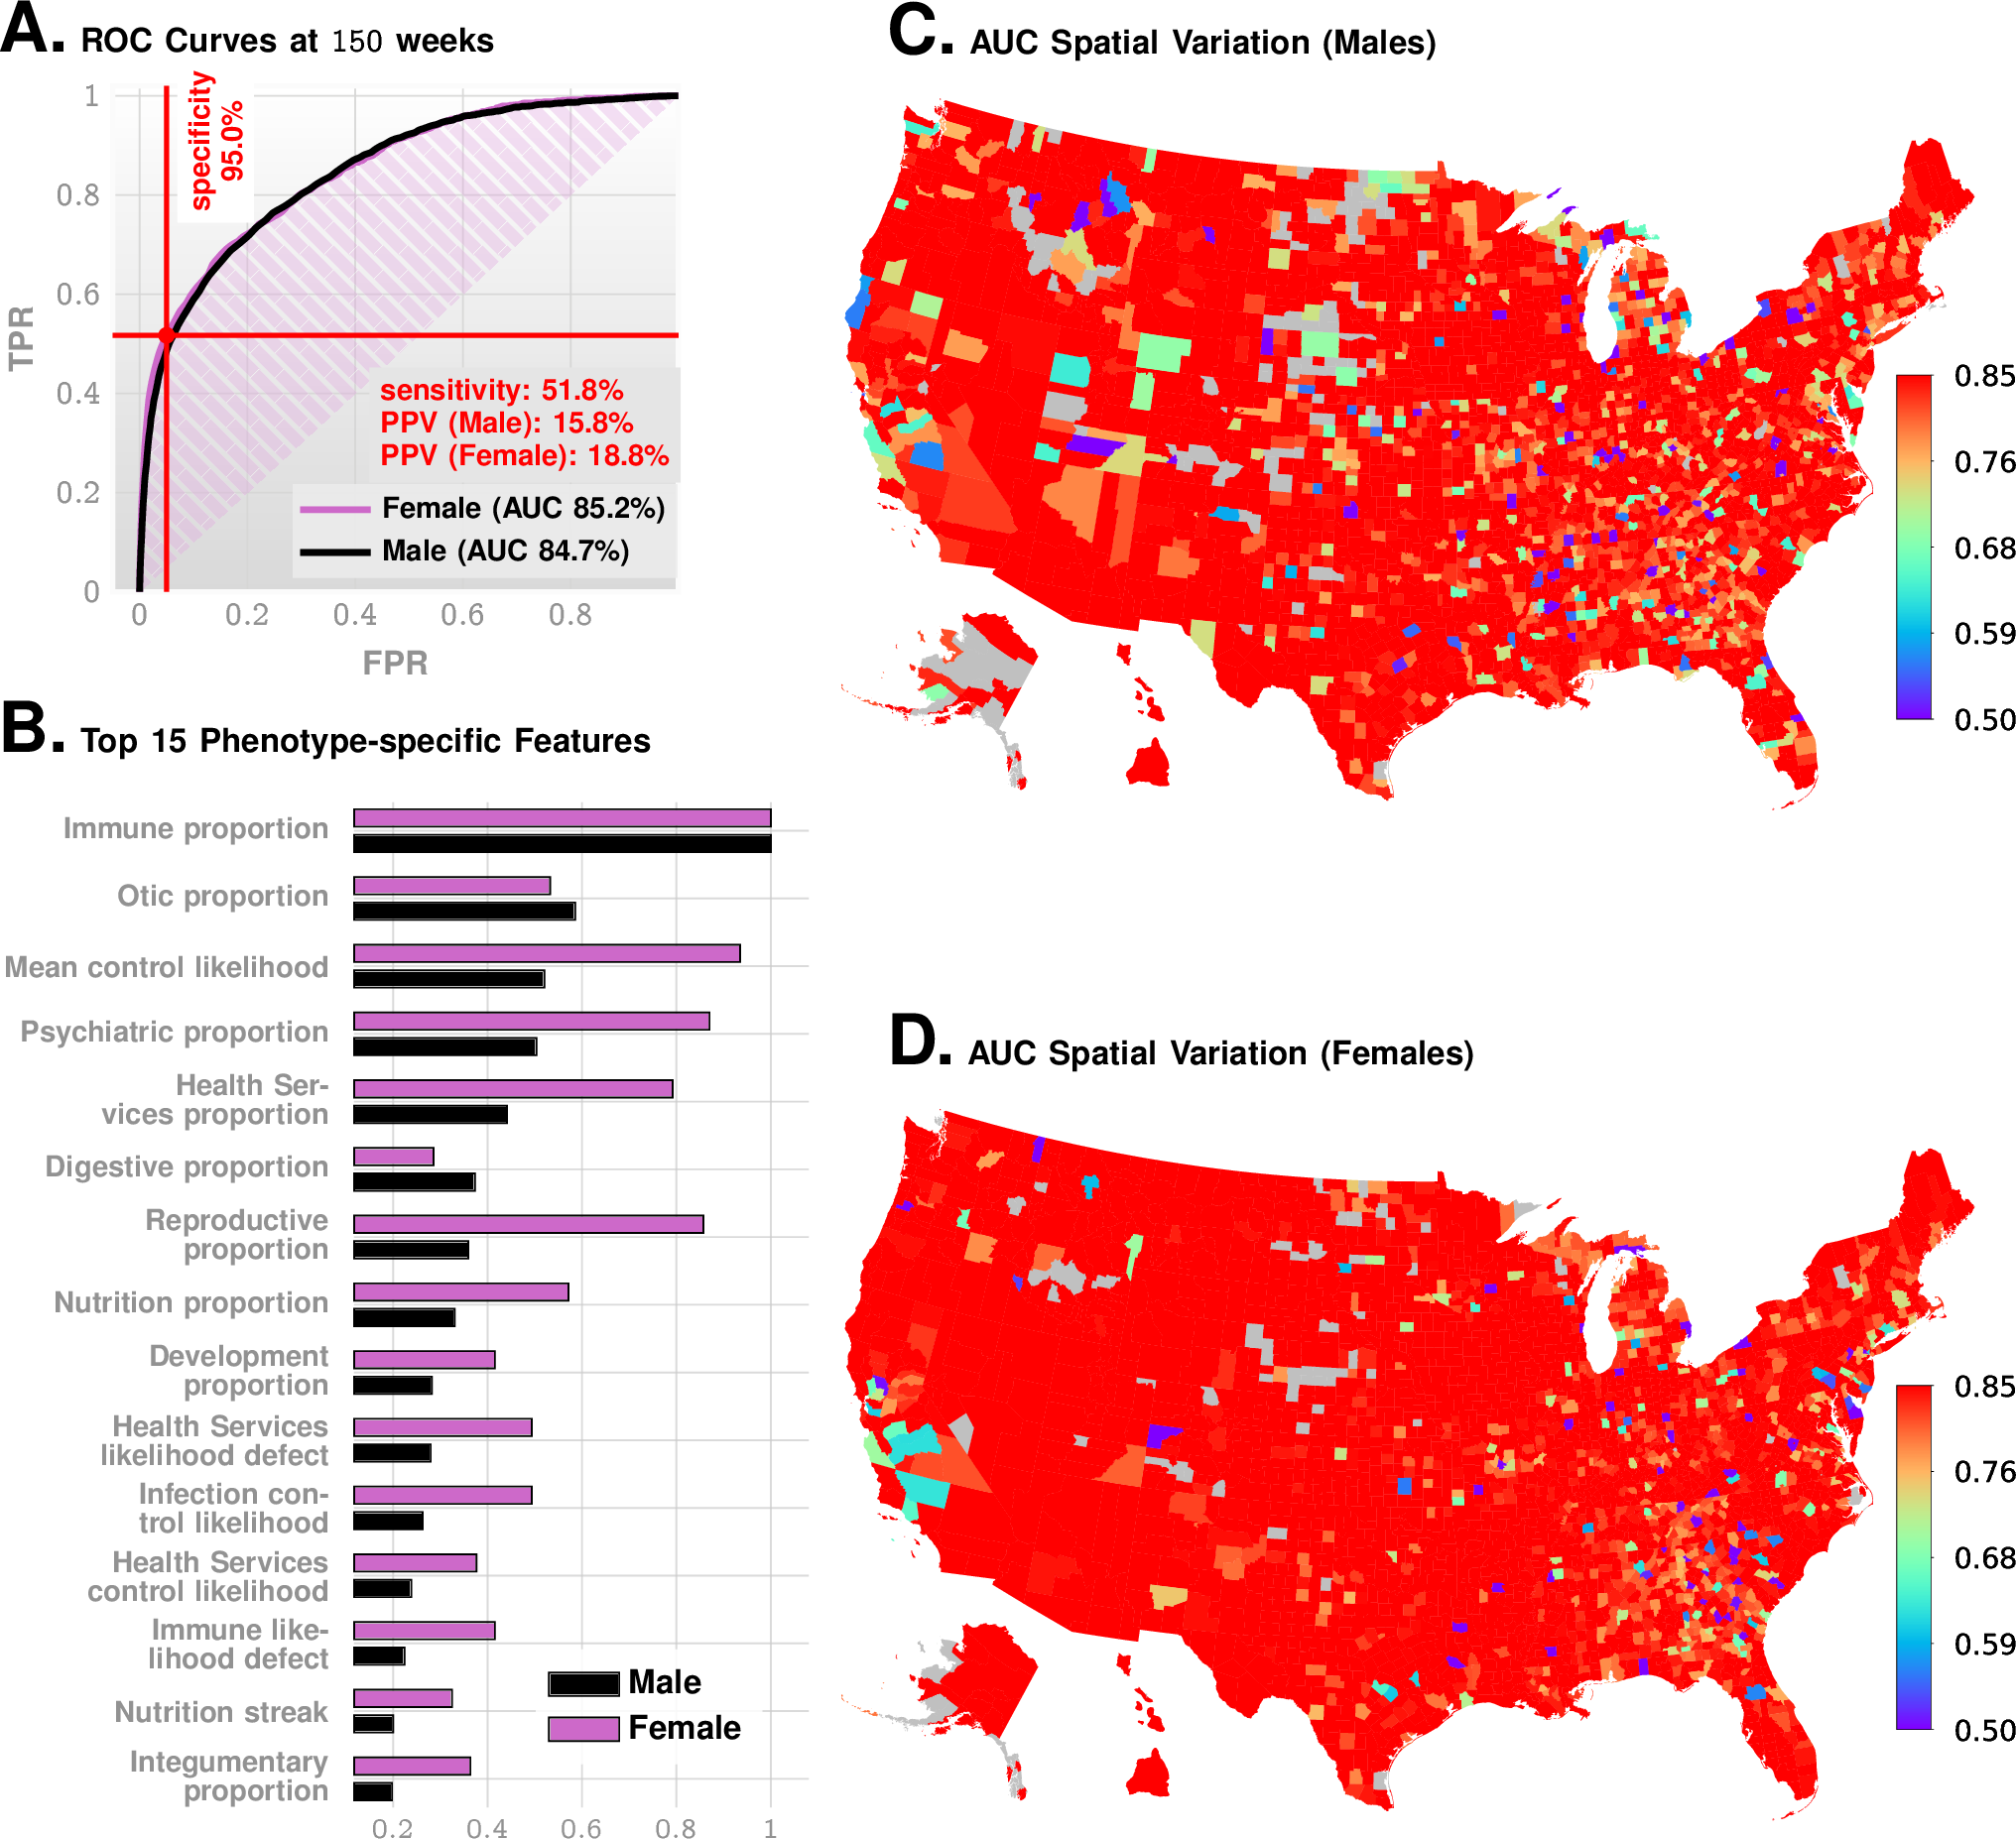
\includegraphics[width=0.8\textwidth]{Figures/main2-figure1.pdf}};

    \end{tikzpicture}
     \vspace{-10pt}

  \captionN{Panel A:  ROC curves. Panel B: feature importance inferred by our prediction pipeline. The most import feature is related to immunologic disorders, and we note that in addition to features related to individual disease categories, we also have the mean control likelihood (rank 3), which may be interpreted as the average likelihood of the diagnostic patterns in the control category vs the \treatment category. 
     }\label{fig1}
        \vspace{-15pt}

\end{wrapfigure}\textbf{Significance of Specific Aim 2:} 
In our retrospective  preliminary studies~\cite{Onishchenko_2021},  \ZERO supersedes M-CHAT/F  performance~\cite{pmid31562252} on a large  cohort with near-universal screening carried out at the Children's Hospital of Philadelphia (CHOP). However, not having observed the \ZERO and the M-CHAT/F scores jointly for individual patients, our preliminary studies lack  assessment of statistical dependence between the two scores. While the  methodologies  suggest functional independence, specific Aim 2 will investigate this rigorously. Independence from existing tools implies  we can   combine the scores to significantly boost standalone  screening performance.

\textbf{Significance of Specific Aim 3:} Use of comorbidity patterns to estimate risk might help reduce the subjective component in questionnaire-based screening tools, resulting in reduced effect of potential language and cultural barriers in diverse populations~\cite{hyman2020identification}. With a significant portion of the  cohort expected to be African Americans and Hispanics in our primary care clinic, we  will be able to explicitly investigate these questions.

\textbf{Significance of Specific Aim 4:} 
Despite   advances in charting  heritability~\cite{Satterstrom484113,sandin17},
efforts to  identify  causal biomarkers  have had limited success~\cite{pmid29691724,pmid29307081}. While   $100-1000$ genes might modulate ASD risk~\cite{pmid26402605,pmid25038753,Satterstrom484113,pmid27891212},   genetics have accounted for a limited number of cases~\cite{pmid18414403}. Suspected sources of environmental  risk  range from maternal infection and inflammation, diet, and  household chemical exposures,  to autoimmune conditions and localized perinatal  inflammation of the central nervous system~\cite{pmid30971960,pmid30941018,pmid29691724,pmid29307081,pmid27351598,pmid26793298,pmid30095240,pmid25681541}. A plurality of   etiologies with converging pathophysiological pathways is also plausible, and we  aim to unravel clues to mechanistic drivers by  categorizing the heterogeneous presentation via signatures buried in longitudinal co-morbidity patterns.
 \subsection{Innovation}
\paragraph*{Paradigm Shift in ASD Screening} Despite extensive documentation of co-morbidities,   a risk estimator that makes reliable predictions for  individuals | based purely on co-morbidity patterns |  has never been reported to  our knowledge. The sparsity of  diagnostic codes in individuals,  the  absence of physiological disorders  that would consistently signal the eventual emergence of ASD symptoms, combined with the heterogeneity of ASD presentation,  make such an endeavor challenging. This \textit{first-of-its-kind}  study proposes to estimate  risk  of a complex neuropsychiatric disease based on longitudinal patterns learned from   large databases of sparse uncurated  medical history. In our preliminary studies, we achieve an out-of-sample AUC exceeding  $80\%$ for  either sex from just over 2 years of age. Our ML algorithm is  fundamentally novel, specifically analyzing sparse, noisy categorical diagnostic sequences. 

\begin{wraptable}[9]{l}{2.5in}
  \vspace{-18pt}
  
   \bf \sffamily \fontsize{8}{8}\selectfont
 \captionN{ASD ICD10 codes used in training}\label{tabtarget}
 \vspace{-10pt}
 
 \hspace{-10pt}
 \begin{tabular}{R{.4in}L{2.75in}}
 F84 &Pervasive developmental disorders\\
 F84.0& Autistic disorder\\
 F84.2 &Rett's syndrome\\
 F84.3 &Other childhood disintegrative disord.\\
 F84.5 &Asperger's syndrome\\
 F84.8 &Other pervasive develop. disorders\\
  F84.9 &Pervasive develop. disorder, unspec\\
   \end{tabular}
 \end{wraptable}
%
Sophisticated analytics to identify children at risk is  of substantial  interest, with  progress being made by several groups~\cite{hyde2019applications,abbas2020multi,duda2016clinical,duda2014testing,fusaro2014potential,wall2012use,wall2012use2}. However, the   focus is often on analyzing questionnaires, and more recently video clips of toddler behavior. Emerging biomraker-based tools~\cite{smith2020metabolomics,howsmon2017classification,hicks2018validation} are not mature enough. Additionally, the inclusion of older children and  small cohort sizes in these studies is problematic. More importantly,  the use of standard  ML on  well-established modalities focuses on mimicing the  physician. In contrast,  \acor exploits under-utilized diagnostic modalities, aiming to model the disease itself, and  not the physician. 
 %###########################################################
%###########################################################
%###########################################################
% %####################################
\subsection{Approach}
We describe our approach in the context of our preliminary retrospective results, outlining  the \ZERO methodology, towards prospective  application in a primary care setting. 

\def\RCOL{\rowcolor{teal!40}}
% ####################################
\begin{wrapfigure}[25]{l}{3.65in}
  \vspace{-15pt}
  
  \centering 
   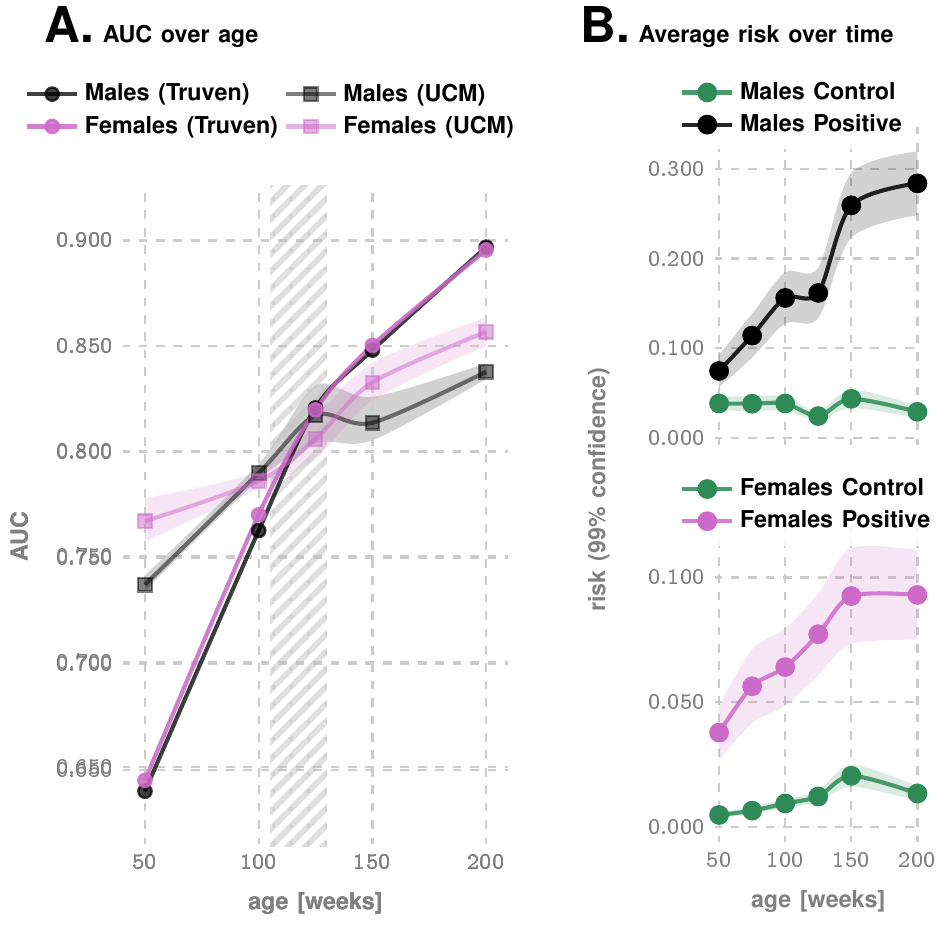
\includegraphics[width=0.5\textwidth]{Figures/perf1}
   \vspace{-15pt}

    \captionN{\acor performance in retrospective studies. Panel A illustrates AUC achieved as a function of
      patient age, for the Truven and UCM datasets: we achieve $>80\%$ AUC for either gender from shortly after 2 years.   Panel B illustrates  risk variation with time for the control and the positive cohorts. % Panel C shows the distribution of the prediction horizon: the time to a clinical diagnosis after inferred  relative risk crosses $90\%$. Panel d illustrates the risk progression of a specific, ultimately autistic male child in the Truven database.
    }\label{fig2}
       \vspace{-15pt}

\end{wrapfigure}
%###########################################################
\subsection*{Source of Electronic Patient Records in Preliminary Studies}
Of the two independent sources of patient records used in our preliminary study,  the primary source used to train our models  is the Truven Health Analytics  MarketScan\textsuperscript{\textregistered} Commercial Claims and Encounters Database for the years 2003 to 2012~\cite{hansen2017truven} (referred to  as the Truven dataset). 
We extracted histories of patients within the age of $0-5$ years, and excluded  patients who do not satisfy the following criteria: 1) At least one code of any available phenotypes is present, 2) Lag between first and last available record for a patient should be at least 15 weeks. These exclusion criteria ensure that we are not considering patients with too few observations to either train on. For training, we analyzed over 4M children ($n=4.4M$), with 30M diagnostic records (16,649,548 for males and  14,318,303  for females with 9,835 unique diagnostic codes).

While the Truven database is used for both training and out-of-sample cross-validation with held-back patient data, our second independent dataset (referred to as the UCM dataset, n=38,012) consisting of de-identified diagnostic records for children treated at the University of Chicago Medical Center between the years of 2006 to 2018, aided in further cross-validation. We considered children between the ages of $0-5$ years, and  applied the same exclusion criteria as the Truven dataset.

Predicting  future ASD diagnosis   is a  binary classification problem: we classify time-stamped sequences of diagnostic codes  into \treatment and \control categories, where the ``\treatment'' category refers to patients eventually  diagnosed with ASD (defined as people with one or more ICD9/10 codes corresponding to ASD in their medical history, See Table~\ref{tabtarget}). 
For learning the differences in longitudinal patterns, we consider  data from birth (or the earliest record) upto the time at which the prediction/screening is done.
We do not pre-select any diagnostic   code based on its  suspected or known comorbidity with ASD.


\subsection*{Modeling \& Prediction}
The significant diversity of diagnostic codes, their typical sparsity,  leads to very few consistent repeats for straightforward  probability calculations,    making this a difficult learning problem. 
We proceed by  partitioning the  disease spectrum into \DXphn\xspace broad  categories, $e.g.$ infectious diseases, immunologic disorders, and endocrinal disorders. Some of these categories comprises a relatively large number of diagnostic codes aligning roughly with the  ICD categories~\cite{hedegaard2019international}.   Each  category yield a single time series over weeks (each week being identified as having a value '0' for no code corresponding to the diagnostic category, or  '1' if some code is present, and '2' if a diagnostic code from any of the other categories is present). 
These time series are  compressed into specialized Hidden Markov Models known as Probabilistic Finite Automata~\cite{CL12g,Chattopadhyay20140826}. These models are inferred separately for each phenotype,  for each sex, and for the control and the \treatment cohorts,  to identify   distinctive average patterns  emerging at the population level. Thus, we infer 
$\DXphn\times 2 \times 2  = \the\numexpr  \DXphn  *2 *2  \relax$  PFSA models in total in the retrosspective studies~\cite{Onishchenko_2021}. Variation in these inferred models across \treatment and \control groups  quantify the divergence of comorbidity patterns with increasing risk~\cite{huang2019data,Onishchenko_2021}. In addition, we use a range of engineered features that reflect various aspects of the patient-specific diagnostic histories, ultimately computing   $\numfeatures$  features    for each patient. These features are  used to train a standard gradient boosting classifier~\cite{ke2017lightgbm} aiming to  map   individual patients  to a raw risk score. $50\%$ of our patients are randomly selected for training with the rest  held-out as a validation set. We measure our performance using  standard metrics including the Area Under the receiver-operating characteristic curve (AUC), sensitivity, specificity, and  the Positive Predictive Value (PPV).

%\subsection*{Feature Importance \& Comorbidity Spectra}
Calculation of the \acor score offers  insights into the relative importance of  comorbidity categories, computed  by estimating the  mean change in the raw risk via random perturbation of %Codes that we used to train the model:
a particular feature: this is the ``feature importance'' shown in Fig.~\ref{fig1}c for top contributing  categories, indicating that immunological, otic, digestive disorders and infections  are   important categories  modulating the \acor score. %In our preliminary studies, we  found excellent disambiguation from other intellectual disabilities such as XXX. \DQS{what other intellectual disabilities}
%
Importantly, our features are  based on data already  available in the past  medical records. We do not demand results from specific tests, or look for specific demographic, bio-molecular, physiological and other parameters; \textit{we use what we get} in the diagnostic history of patients.

% %####################################
The standalone performance in preliminary studies is summarized  in Figs.~\ref{fig1} and \ref{fig2}. 
We achieve an out-of-sample AUC of $82.3\%$ for males and $82.5\%$ for females at $125$ weeks of age for the Truven dataset. In the UCM dataset, our performance is comparable: $83.1\%$ and $81.3\%$ for males and females respectively at $125$ weeks of age. Predictive performance was observed to increase with patient age (ROC curve obtained at 150 weeks shown in Fig.~\ref{fig1}A, and AUC variation with age with 99\% confidence bounds is shown in Fig.~\ref{fig2}A), reaching close to 90\% at around 4 years in the national database. The good agreement of the out-of-sample performance on these independent datasets lends strong support for our claims. The specificity, sensitivity, PPV trade-offs are shown in Table~\ref{tabssp}. We enumerate the top $15$ predictive features in Fig.~\ref{fig1}B. 
We also computed the county-specific performance of \acor, and we got nearly uniform performance across the country for both sexes~\cite{Onishchenko_2021}. 
%
%
%Fig.~\ref{fig2}A illustrates the variation of the  AUC  with increasing age of the subjects plotted with 99\% confidence bounds, indicating the predictive performance increases with age.
We find that while the AUC gradients are slightly different in the two datasets are comparable.

%####################################
\begin{wraptable}[9]{l}{2.5in}  
  \centering
  \vspace{-19pt}
  
\captionN{Standalone \acor performance (M-CHAT/F: sensitivity=$38.8\%$,specificity=$95\%$, PPV=$14.6\%$)}\label{tabssp}
\fontsize{8}{8}\selectfont
  \vspace{-10pt}
 \begin{tabular}{L{.27in}|L{.27in}|L{.25in}|L{.25in}|L{.45in}}
\hline
spec.&sens.&PPV&sex&dataset\\\hline
% 100&0.92&0.39&0.14&F&UCM\\\hline
% 100&0.95&0.39&0.19&M&UCM\\\hline
% 100&0.93&0.39&0.13&F&Truven\\\hline
% 100&0.91&0.39&0.10&M&Truven\\\hline
%\RCOL 112&0.94&0.35&0.17&F&UCM\\\hline
\RCOL 0.93&0.39&0.16&F&UCM\\\hline
\RCOL 0.95&0.39&0.20&M&UCM\\\hline
\RCOL 0.96&0.39&0.22&F&Truven\\\hline
\RCOL 0.95&0.39&0.17&M&Truven%\hline
% 150&0.94&0.39&0.19&F&UCM\\\hline
% 150&0.98&0.39&0.34&F&Truven\\\hline
% 150&0.97&0.39&0.26&M&Truven\\\hline
% 150&0.97&0.39&0.26&M&UCM\\\hline
\\\hline
\end{tabular}
\end{wraptable}  
%####################################
We plot the raw risk over time for males and females for the out-of-sample control and \treatment cohorts in Fig.~\ref{fig2}B. Notably, averaged over the population,   the risks differ  from $50$ weeks showing that early disambiguation is possible. Guthrie $\etal$~\cite{pmid31562252}  has  demonstrated that  as a nearly universal screening tool (n=20,375) M-CHAT/F (between 18-26 months) has a sensitivity of 38.8\%, specificity of 94.9\% and PPV of 14.6\%, which suggests  (See Table~\ref{tabssp}) that our approach produces a  superior PPV (exceeding M-CHAT/F PPV by at  $14\%$ (14.1-33.6\%) when sensitivity and specificity are held at comparable values around the age of 26 months ($\approx 112$ weeks). 

%#################################### 
\begin{wraptable}[9]{l}{4.2in}
  \centering
  \vspace{-15pt}
  
\captionN{\acor Performance at  26 months  Conditioned on M-CHAT/F}\label{tabboost}
\fontsize{8}{8}\selectfont

\vspace{-4pt}

\begin{tabular} {L{.2in}|L{.2in}|L{.2in}|L{.2in}||L{.275in}|L{.285in}|L{.285in}||L{.275in}|L{.285in}|L{.285in}}
\hline
\multicolumn{4}{c||}{\cellcolor{lightgray!60}M-CHAT/F Outcome}  & \multicolumn{3}{c||}{\mnp{.9in}{\vskip .2em  perf. (Truven)\vskip .2em  } }&\multicolumn{3}{c}{\mnp{1in}{\vskip .2em  perf. (UCM)\vskip .2em }} \\\cline{0-9}
 0-2  NEG & 3-7  NEG & 3-7  POS & $\geq  8$  POS & \multirow{2}{*}{\mnp{.1in}{speci-ficity}} & \multirow{2}{*}{\mnp{.1in}{sensi-tivity}} &\multirow{2}{*}{PPV}& \multirow{2}{*}{\mnp{.1in}{speci-ficity}} & \multirow{2}{*}{\mnp{.1in}{sensi-tivity}} & \multirow{2}{*}{PPV}  \\\cline{0-2}
\multicolumn{4}{c}{\cellcolor{lightgray} specificity choices}  & & & &&&\\\hline 
  0.48&0.87&0.97&0.99&0.98&0.432&0.331&0.98&0.355&0.289\\\hline 
0.38&0.54&0.94&0.98&0.95&0.736&0.203&0.95&0.628&0.178\\\hline \\\hline
\end{tabular}
\vspace{-18pt}

\end{wraptable}  
%####################################
In Aim 2, we aim to combine \acor amd M-CHAT/F  via a conditional choice of  sensitivity/specificity trade-offs. In our preliminary studies, we use Guthrie $\etal$~\cite{pmid31562252}'s estimate of the population distribution of M-CHAT/F scores to estimate this conditional trade-off, and find this boosts overall performance significantly, with  a PPV $\approx 30\%$  across datasets, or a sensitivity close to or exceeding $50\%$, when we restrict specificities to above $95\%$ (See Table~\ref{tabboost}).


\subsection*{Inferred Co-morbidity Patterns \& Normalized Prevalence Comparison}
% ###########################################################

\begin{figure*}[t]
  \tikzexternaldisable
  \vspace{-10pt}

  \begin{tikzpicture}[font=\bf\sffamily\fontsize{8}{8}\selectfont,scale=.7]
    \node[label={[yshift=-.5in]90:{\Large A.} Males}] (A) at (0,0) {
      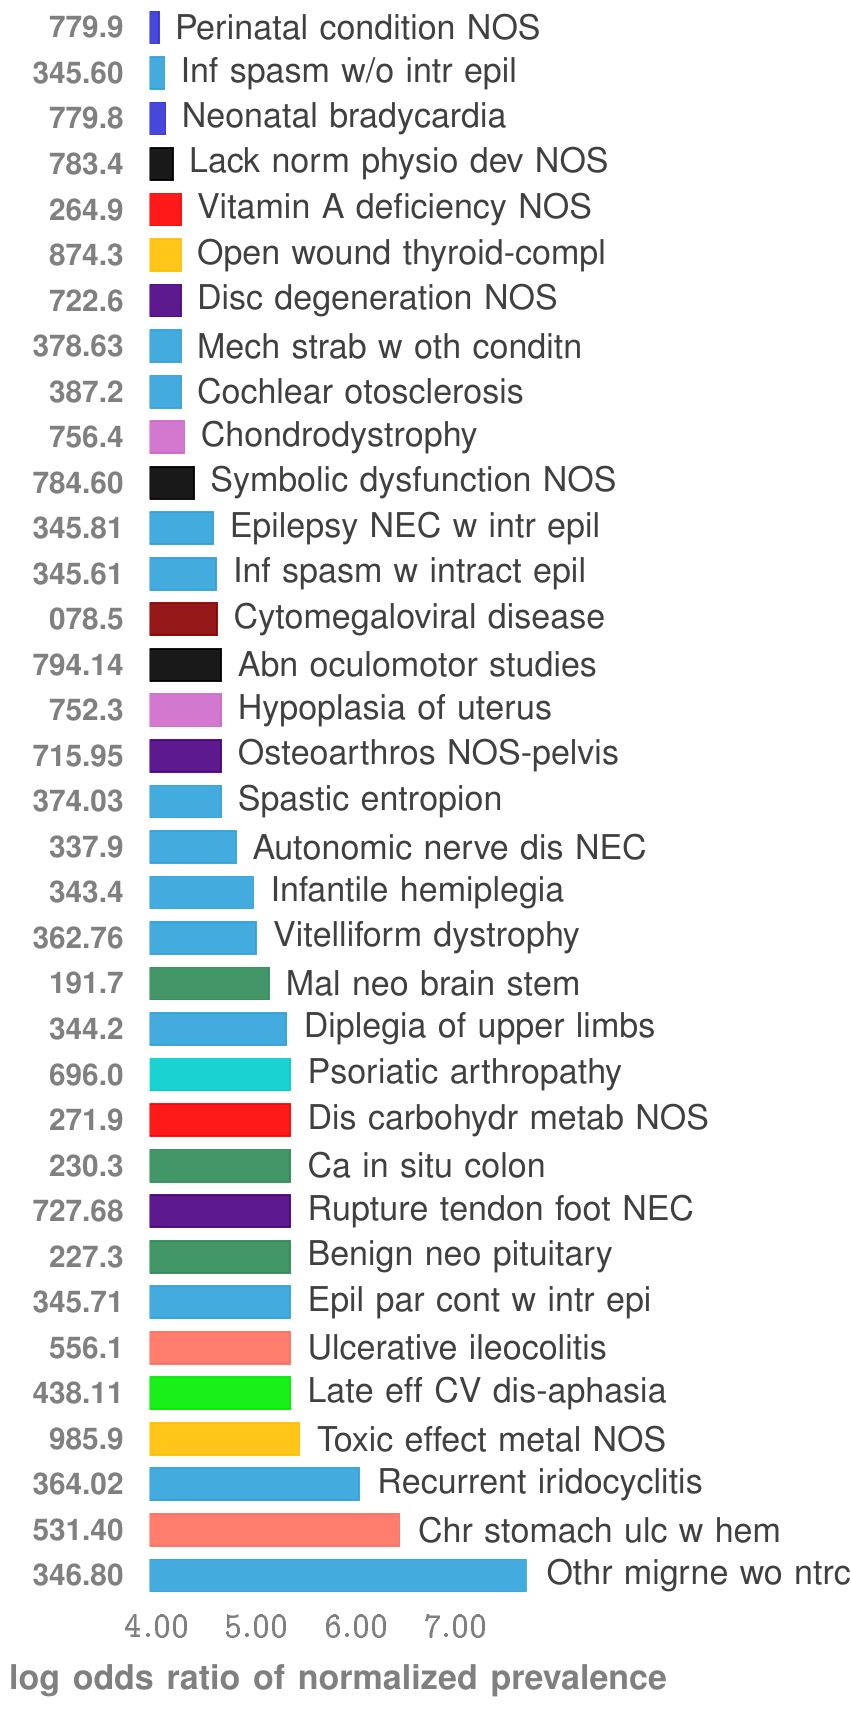
\includegraphics[height=6in,angle=90]{Figures/bars1}};
    \node[anchor=west] (B) at (A.east) {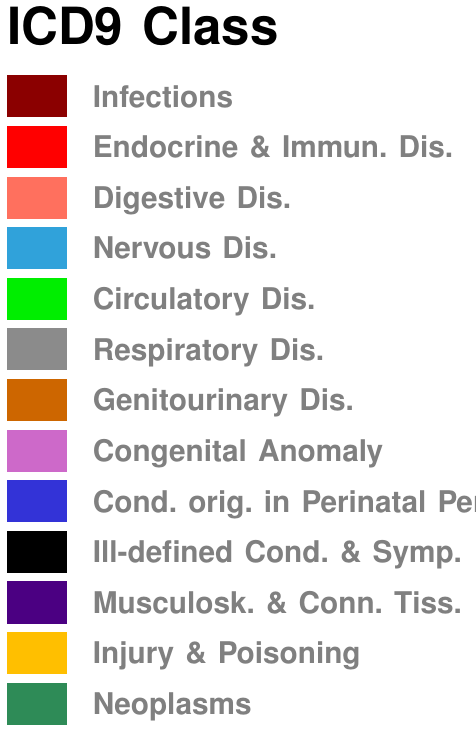
\includegraphics[height=2in,angle=0]{Figures/bars2}};
  \end{tikzpicture}
  \vspace{-20pt}
  
  \captionN{Difference in occurrence frequencies of diagnostic codes between true positive (TP) and true negative (TN) predictions in males. The color coding shows the disease categories of the co-morbidities.}\label{fig3}
    \vspace{-10pt}

\end{figure*}
% ###########################################################
The predictive ability of our pipeline arises from the difference in patterns of co-morbid disorders between the \treatment and the control cohorts: the diagnostic history of individual patients is not random and hides key signatures to future neuropsychiatric outcomes. As an illustrative example, a single random patient from the Truven database is illustrated in Fig.~\ref{fig2}D.
Color-coding the diagnoses according to the broad ICD9 disease categories reveals that for this specific individual, infections and immunological disorders are experienced early to a much higher degree compared to other diseases, and diseases of the nervous system and sensory organs, as well as ill-defined symptoms dominate the latter period. This suggests the necessity of a deeper interrogation of the structure of co-morbid patterns, which we carried out in our preliminary investigations, as described next.
%
While the ASD co-morbidity burden  is reported to be high for nearly the entire spectrum of  physiological disorders, in our preliminary we find novel association patterns in normalized prevalence | the odds of experiencing a specific disorder, particularly in the early years (age~$<3$ years), normalized over all unique disorders experienced in the specified time-frame. Additionally, we only focus on  the true positives in the \treatment cohort and the true negatives in the control cohort. This  allows us to investigate  patterns that correctly disambiguate future ASD status, $i.e.$, strongly favor one outcome over the other at the individual level (as opposed to population-level prevalence rates), as shown in  Fig.~\ref{fig3} for males.

\begin{wrapfigure}[24]{l}{2.25in}
  \vspace{-30pt}
  
  \hspace{-10pt}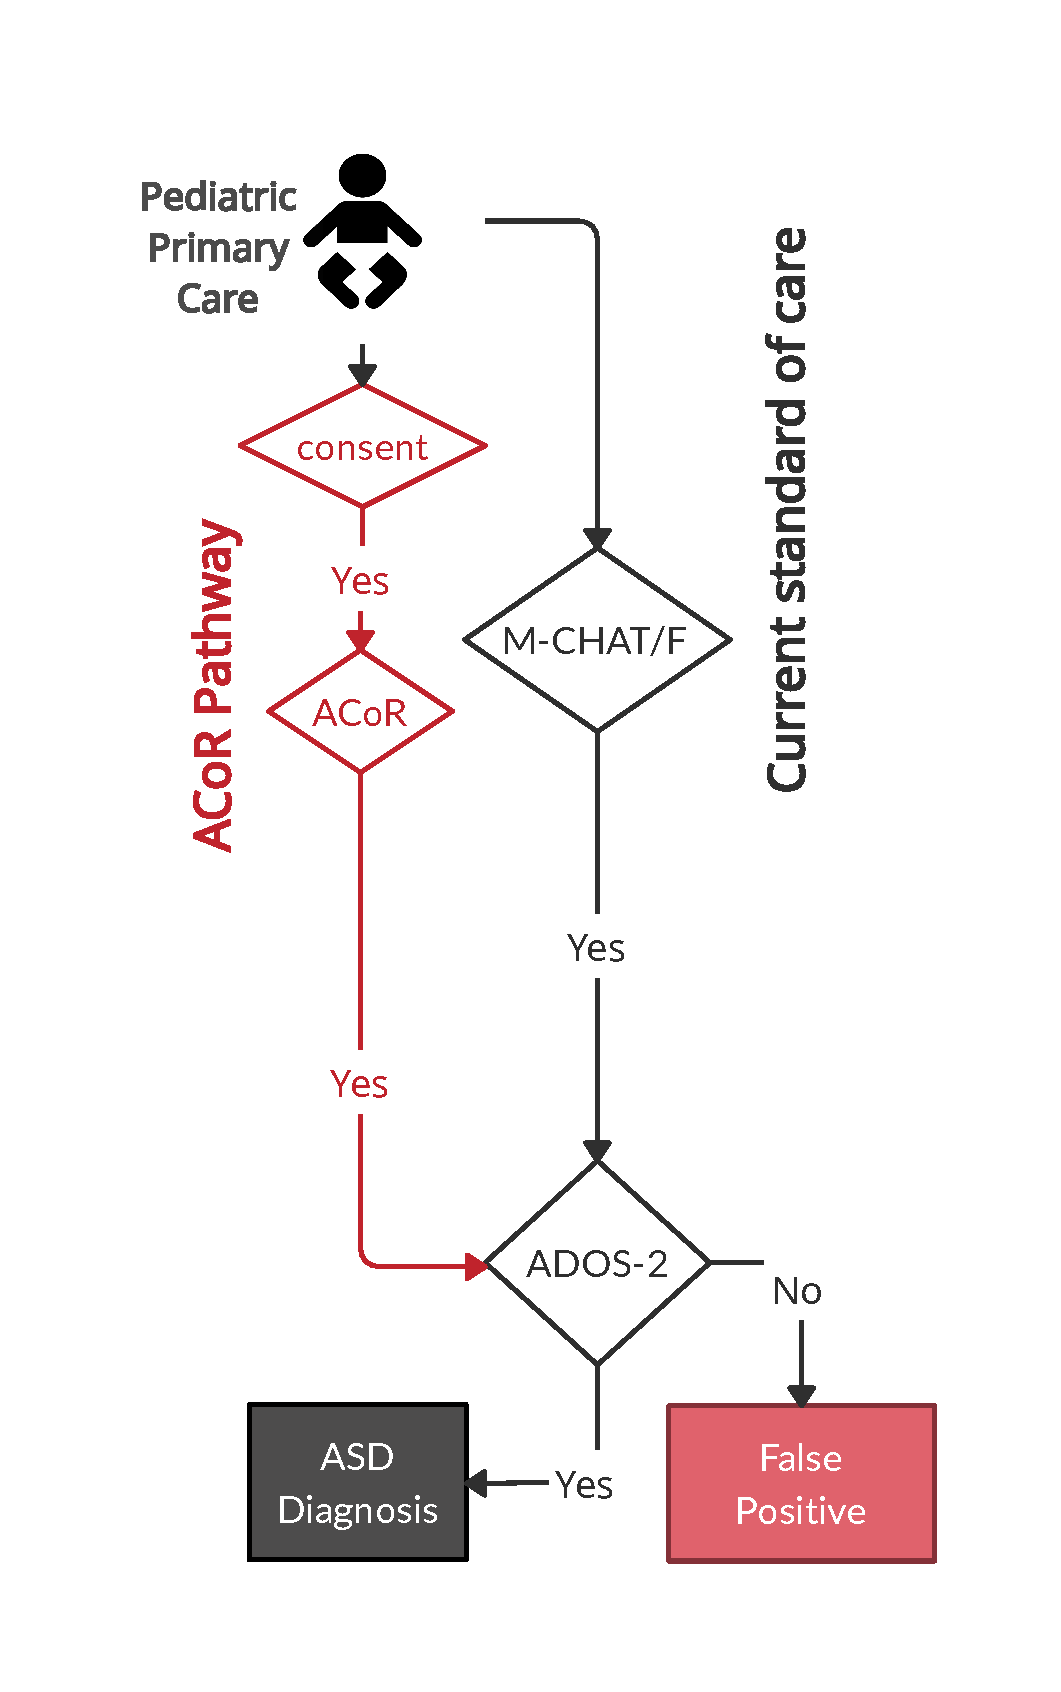
\includegraphics[width=2.75in]{Figures/flowx}
  \vspace{-30pt}
  
  \captionN{Patient processing logic: Note we have parallel pathways through M-CHAT/F and \acor, and
  a flag in either triggers the ADOS-2 evaluation.}\label{figflow}
\end{wrapfigure}\subsection*{Disambiguation From Unrelated Psychiatric Phenotypes}
%
In our retrospective analyses,  we investigated if we can discriminate between ASD and other unrelated psychiatric phenotypes, by restricting the  control  cohort in validation to  patients with at least one psychiatric code other than ASD. We get very high discrimination reaching AUCs over $90\%$ at $100-125$ weeks of age~\cite{Onishchenko_2021}, which establishes that our pipeline is indeed largely specific to ASD. 

% \begin{wrapfigure}[13]{l}{2.2in}  
%   \centering
%   \vspace{-17pt}
  
%   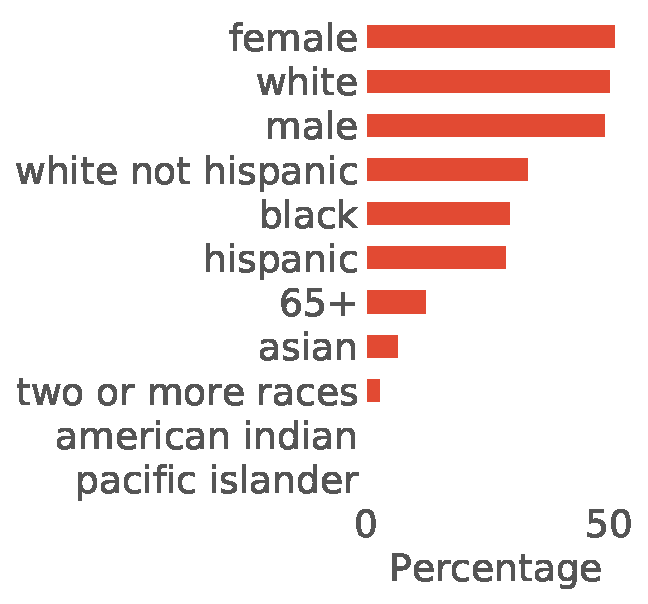
\includegraphics[width=2.18in]{Figures/demo}
%   \vspace{-15pt}

  
% \caption{Expected demographic makeup  in proposed study}\label{tabdemo1}

% \end{wrapfigure}
\subsection*{Addressing Uncertainty in EHR Records}
Recent changes in diagnostic practice, $e.g.$ increased diagnoses from individual clinicians versus prior eras that only allowed diagnosis from the gold-standard multi-disciplinary teams can  increase observed   prevalence, and  raises the possibility that  some diagnostic codes pertaining to ASD in medical history databases could be arising from less restrictive workflows, and  are susceptible to increased uncertainty.  In our preliminary study, we verified that restricting the \treatment cohort to children with at least two  distinct ASD diagnostic codes in their medical histories instead of one, has little impact on  out-of-sample predictive performance.
 
We also found that the density of diagnostic codes in a child's medical history by itself is somewhat predictive of a future ASD diagnosis, but not at clinically significant levels.


\subsection*{Research Design}

 To achieve the specific aims, we will gather data from both the child and the primary caregiver (standard care) in the participating primary care clinic. Eligible patients at the Department of Pediatrics, University of Chicago (patients who present for a well-child visit between 16-26 months or any other non-emergency reason) will be asked for consent for access to their past medical history for carrying out the ACoR screen. If there is a flag either in M-CHAT/F or if M-CHAT/F is borderline with a flag in ACoR, the pediatrician will inform parents of a potential elevated risk of ASD, and offer to schedule for an ADOS-2 evaluation. The ADOS-2 evaluation triggered by ACoR flags will be at no cost to the patient. For all assessments, basic demographic information, recruitment site, medications and diagnoses assigned by the current clinical treatment team, will be obtained from the parent/caregiver and medical record. The sequential  steps in the study (Fig.~\ref{figflow}) are as follows: 1) Pediatric clinic team (led by Dr. Mitchell) will administer M-CHAT/F to incoming children with 16-26 months and procure consent, 2) The PI’s team will compute individual ACoR, 3) If flagged by either  M-CHAT/F or \acor as high risk for ASD, the patients will be scheduled for ADOS-2 evaluation overseen by Dr. Smith, Dr. Msall  and supporting team, and finally, 4) The evaluation scores will be analyzed by PI and his team.
The feasibility of proposed  design has been validated with the same study team under a modest intramural pilot grant, with low sample size (Of 5 \acor flags produced in this pilot, all were diagnosed with ASD by ADOS-2).
% The limited scope of this project implies that we need to be careful about the number of ADOS-2 referral generated due to \ZERO, particularly since ADOS-2 evaluations involve significant resource and cost.

\begin{wraptable}[13]{l}{1.65in}
  \fontsize{8}{8}\selectfont

  \vspace{-18pt}
  
  \captionN{Expected population demographics}\label{tabdemo}
  \begin{tabular}{L{.753in}L{.53in}}
  \rowcolor{lightgray}  Sex & \\
Male & 53.6\%\\
       Female & 46.6\%\\\hline\rowcolor{lightgray}  Race & \\
                Black/African-Am & 73.2\%\\
                                   White & 18.2\%\\
    Asian &3\%\\\hline
    \rowcolor{lightgray}  Ethnicity & \\
  Hispanic & 7.9\% \\
  Non-Hispanic & 91.8\% 
\end{tabular}
\end{wraptable}
\subsection*{Cohort Selection: Inclusion and Exclusion Criteria}
% Our expected cohort is diverse ), with greater than 70\% of participants expected to be African-American, as surmisd from the UCM data in our retrospective analysis.
% Sample size for this study is mainly determined by the number of children served by the particpating pediatric clinics within the ages of 16-26 months. We expect to recruit approximately 3000 children per year. Our inclusion criterion is only the age bracket, and children who already have a ASD diagnsosis will be excluded. Additionally, children with less than 5 diganostic codes in their medical history will be excluded.

We are aiming to validate a universal screening protocol for ASD risk. As such, we do not plan to select patients based on gender or demographic criteria, and plan to carry out ongoing recruitment at the pediatric clinic involved in this study throughout the study timeline, as long as the patients are within the target age bracket of 16-26 months.  Nevertheless, the population from which our patients will be drawn is diverse (See Fig.~\ref{tabdemo}), with greater than 70\% of the patients being non-Caucasian. The split between male and females is expected to be approximately even (54\% males to 46\% females), as estimated from past patient population characteristics (in the age group of interest) treated at the University of Chicago Medical center. Estimating from the number of well-child visits at the pediatric clinic involved in this study, we estimate that our sample size will be approximately 3000. Hence our inclusion criteria is: age within 16-26 months, and our exclusion criteria are: 1) children who already have a ASD diagnsosis will be excluded. 2) children with less than 5 diganostic codes in their medical history.


% (producing approximately 300 ADOS-2 referrals from M-CHAT/F at no cost to the project) who will be evaluated via both the MCHAT-F screening  during wellness visits at the 1 year, 1.5 year and 2 year mark, and the \ZERO algorithm applied to their diagnostic history on file. Additional inclusion criteria: Child has diagnostic history on record with at least 5 diagnostic codes, and the first code is at least from 15 weeks in the past. Additional exclusion criteria: Diagnostic history only consists of health service contact codes.

% Beyond the evaluation of $\approx 300$ children as a part of standard clinical workflow, we will evaluate $100-120$ children at no cost to the patient family, to evaluate the efficacy of \acor when M-CHAT/F is borderline (and does not trigger downstream diagnostic evaluation by itself).

\subsection*{Sample Size for ADOS-2 Evaluations} \acor screening conditioned on M-CHAT/F is expected to have a sensitivity $>70\%$ and a PPV $>20\%$, implying that we expect to have prevalence x 0.7 x 3000 x (1/0.2) flags at 95\% specificity. Assuming a 10\% prevalence (consenting parents might have observed some concerning developmental issues, and thus bias the sample from population prevalence of ASD), we determine that we would need to do about 300 ADOS-2 evaluations per year. We would also investigate higher sensitivity operation for \acor at 90\% (since \acor allows for a choice of a range of operating points on the ROC curve), where up to 500 ADOS-2 evaluations per year would suffice. From estimated confidence bounds on \acor performance, this sample size estimates are sufficient to achieve greater than 80\% power at 5\% signifiance.

\subsection{Study Interventions}
No intervention is planned. Outcomes are  efficacy and applicability of \ZERO.
\subsection*{Risk To Patients}
Since no intervention is planned, and outcomes are efficacy and applicability of ACoR, patients are expected to
suffer limited negative impact from the additional screen. For some borderline cases might be flagged due to
false positives, which may be viewed as a risk. However, the potential benefits, including significant reduction in
false positives, outweighs the temporary anxiety on part of the care-givers on a false positive flag. It is
conceivable that a false-positive flag gets a positive diagnostic evaluation in the subsequent ADOS-2 evaluation,
and actually gets a clinical diagnosis of ASD. This is unlikely, but is theoretically a risk to patients.
% Adequacy of Protection Against Risks:

The upper bound on the likelihood of a false flag from ACoR, where the M-CHAT/F is negative is estimated to be $\sim$7\% of the total study sample. Given that ADOS evaluation has been reported in some studies to have about $\sim$15\% false positive rate, the risk of a positive diagnosis from ADOS-2 arising triggered by the false flag from ACoR expected to be $\sim$1\% of the
total sample size. However, the ADOS-2 evaluation results will be analyzed by Drs. Smith and Msall (clinical evaluation by
experienced clinicians decreases false positive rate) to minimize the odds of such false positives being recorded as a
clinical diagnosis of ASD for a patient. Thus the actual odds of such an event is expected to be very small. 


\subsection*{Procedures} The ADOS-2 evaluations triggered by \acor will be at no cost to the patient. Patients who are flagged by M-CHAT/F alone will follow standard care, and will not be charged to the project. All study procedures and consent forms will be approved by the University of Chicago Institutional Review Board (IRB).  For all assessments, basic demographic information, recruitment site, medications and diagnoses assigned by the current clinical treatment team, will be obtained from the parent/caregiver and medical record.

\subsection*{Data and Resource Management} Data collection forms for demographic and clinical history data, database design and data management procedures will be designed, created and conducted at the University of Chicago under the
direction of Dr. Smith and Prof. Chattopadhyay. Demographic and clinical history data will be collected and entered into an HIPAA compliant secure databases.  De-identified  data will be deposited to NDA following data harmonization guidelines, and will also be made available in Zenodo. 


\clearpage
\normalem 

%\bibliographystyle{naturemag}
%\bibliography{aut,BibLib1}

\end{document}


% LocalWords:  neurobiological morbidities modality
 